%!TEX root = lot3.tex

%%%%%%%%%%%%%%%%%%%%%%%%%%%%%%%%%%%%%%%%%%%%%%%%%%%%%%%%%%%%%%
%%JULIEN
\begin{tikzpicture} %Recto
	%Fond
    \node[anchor=south west,inner sep=0] (carte) at (0,0) {
\includegraphics[width=7.1 cm, height=9.6 cm]{fonds/noir.png}};
    \node[anchor=center] at (carte.center) {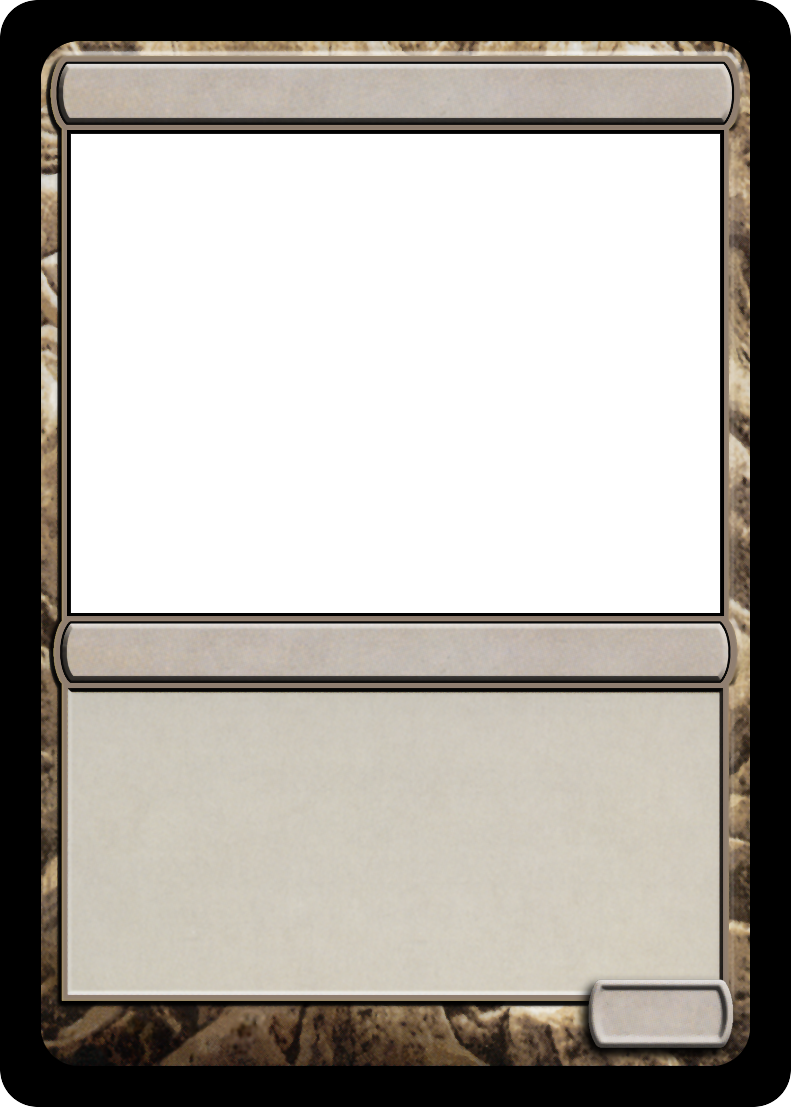
\includegraphics[width=\cardwidth cm, height=\cardheight cm]{fonds/fond_personnage.png}};

    %Titre
	\node[anchor=center] at (\titleX,\titleY) {\titlefont Julien};

	%Image
	\node[anchor=center] at (\imageX,\imageY) {
\includegraphics[width=\imageWidth px, height=\imageHeight px]{images/Hero_Julien.jpg}};
	\node[anchor=center] at (6.1,4.5) {
\includegraphics[width=10 px, height=10 px]{fonds2/violet.jpg}};

	%Type
	\node[anchor=center] at (\typeX,\typeY) {\typefont Personnage Unique};

	%Description
	\node[anchor=north west, text width=5.6cm] (description) at (\descriptionX,\descriptionY) {\descriptionfont\setsize{6}(Génie incompris). Si vous êtes Julien, posez cette carte devant vous au début de la partie. Si le cryptologue ou le développeur n'est pas présent à la fin de votre tour,  jouez un tour supplémentaire avec l'un d'eux. Lorsqu'un malus est appliqué à l'un des joueurs, sur une révélation impaire celui-ci dit "c'est pour Julien", et le malus est détourné sur vous.\par};

	%Punchline
	\node[anchor=north west, text width=5.6cm, below = 1pt of description] (punchline) {\punchlinefont\setsize{6}{\bf (Permanent) Tout comme le bord de cette carte, vous êtes en or.}\par};

	%Separateur !!!!!PAS TOUCHE!!!!!
	\fill[black,path fading=west] (description.south west) rectangle (punchline.north);
	\fill[black,path fading=east] (punchline.north) rectangle (description.south east);

	%Numéro !!!!!PAS TOUCHE!!!!!
	\node[anchor=center] at (\numberX,\numberY) {\numberfont **/**};
\end{tikzpicture}\versoperso %Verso

%%%%%%%%%%%%%%%%%%%%%%%%%%%%%%%%%%%%%%%%%%%%%%%%%%%%%%%%%%%%%%
%%ERIC
\begin{tikzpicture} %Recto
	%Fond
    \node[anchor=south west,inner sep=0] (carte) at (0,0) {
\includegraphics[width=7.1 cm, height=9.6 cm]{fonds/noir.png}};
    \node[anchor=center] at (carte.center) {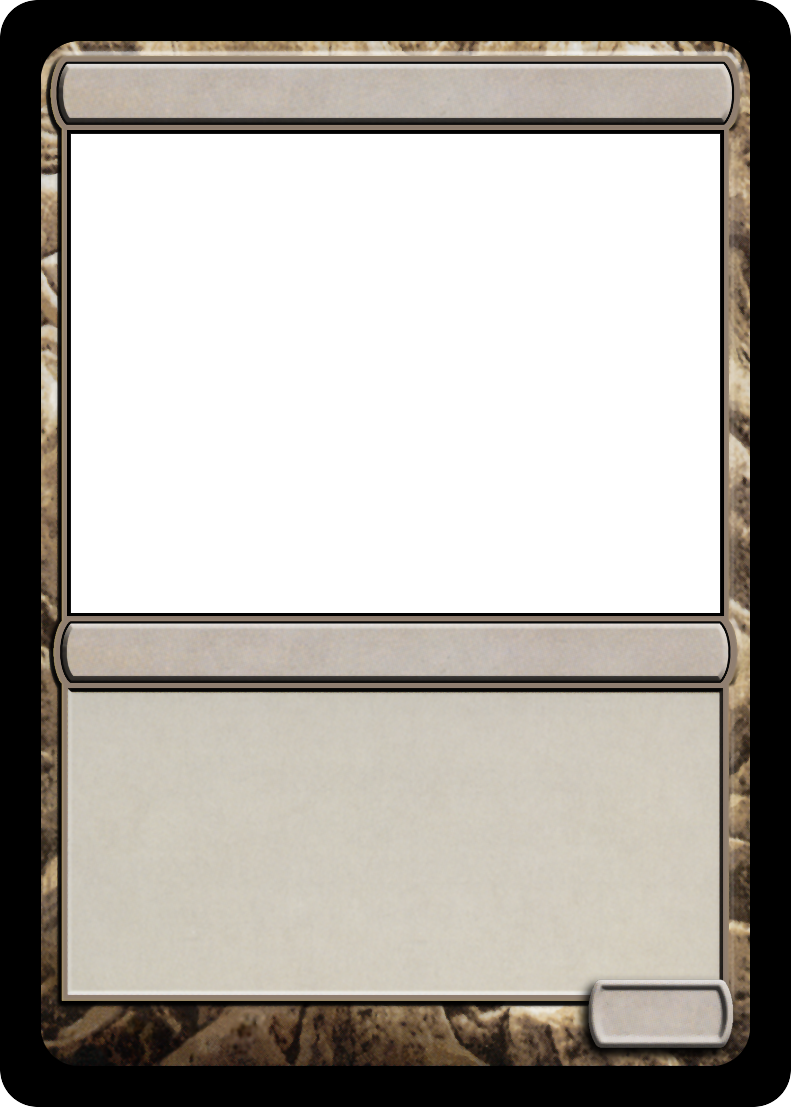
\includegraphics[width=\cardwidth cm, height=\cardheight cm]{fonds/fond_personnage.png}};

    %Titre
	\node[anchor=center] at (\titleX,\titleY) {\titlefont Eric};

	%Image
	\node[anchor=center] at (\imageX,\imageY) {
\includegraphics[width=\imageWidth px, height=\imageHeight px]{images/eric.jpg}};
	\node[anchor=center] at (6.1,4.5) {
\includegraphics[width=10 px, height=10 px]{fonds2/violet.jpg}};

	%Type
	\node[anchor=center] at (\typeX,\typeY) {\typefont Personnage Unique};

	%Description
	\node[anchor=north west, text width=5.6cm] (description) at (\descriptionX,\descriptionY) {\descriptionfont\setsize{6}(Cloud Manager et Chat de goutière). Si vous êtes Eric, posez cette carte devant vous au début de la partie. Vous devez prendre la carte manager si elle a été laissée de côté à ce tour pour préparer le plan de charge.
	Vous pouvez échanger une carte de votre main contre deux cartes de la défausse en début de tour.\par};

	%Punchline
	\node[anchor=north west, text width=5.6cm, below = 1pt of description] (punchline) {\punchlinefont\setsize{5}{\bf "Du caca de gitan dans le sanibroyeur, mais non! You Walsh it, you Walsh it, it smells like a flower !"}\par};

	%Separateur !!!!!PAS TOUCHE!!!!!
	\fill[black,path fading=west] (description.south west) rectangle (punchline.north);
	\fill[black,path fading=east] (punchline.north) rectangle (description.south east);

	%Numéro !!!!!PAS TOUCHE!!!!!
	\node[anchor=center] at (\numberX,\numberY) {\numberfont **/**};
\end{tikzpicture}\versoperso %Verso
%%%%%%%%%%%%%%%%%%%%%%%%%%%%%%%%%%%%%%%%%%%%%%%%%%%%%%%%%%%%%% PMO

%%%%%%%%%%%%%%%%%%%%%%%%%%%%%%%%%%%%%%%%%%%%%%%%%%%%%%%%%%%%%%
%%MATTHIEU
\begin{tikzpicture} %Recto
	%Fond
    \node[anchor=south west,inner sep=0] (carte) at (0,0) {
\includegraphics[width=7.1 cm, height=9.6 cm]{fonds/noir.png}};
    \node[anchor=center] at (carte.center) {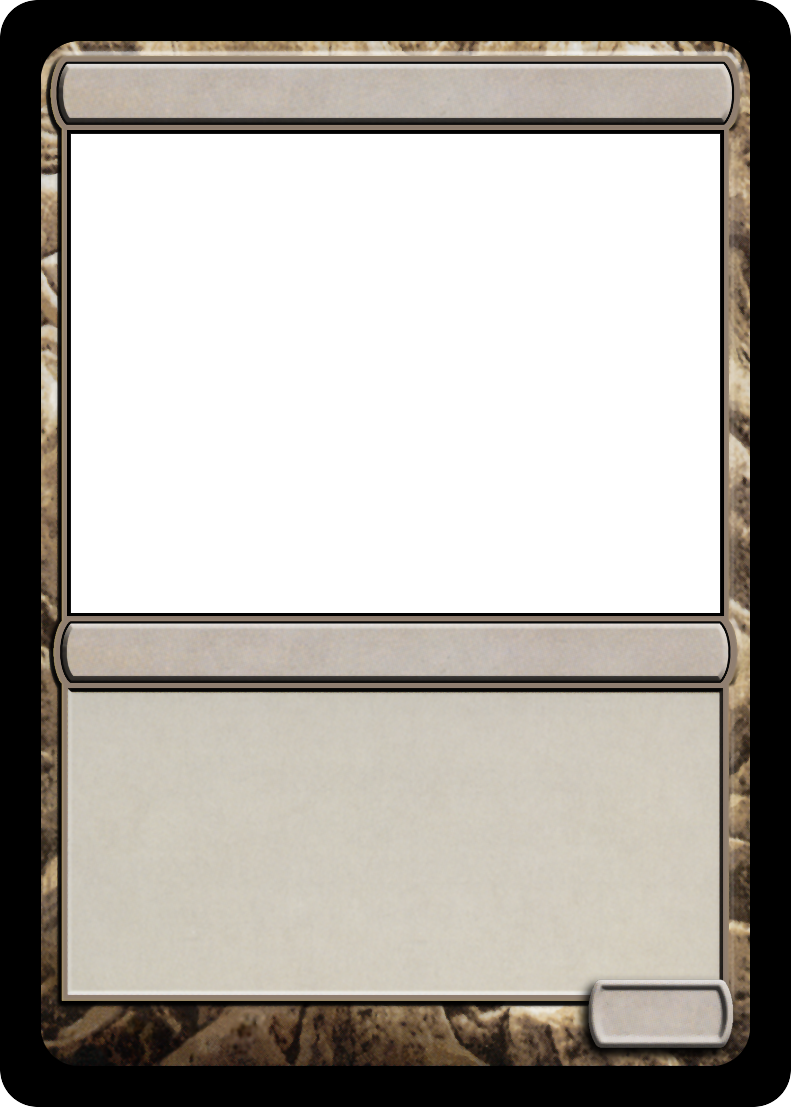
\includegraphics[width=\cardwidth cm, height=\cardheight cm]{fonds/fond_personnage.png}};

    %Titre
	\node[anchor=center] at (\titleX,\titleY) {\titlefont Matthieu};

	%Image
	\node[anchor=center] at (\imageX,\imageY) {
\includegraphics[width=\imageWidth px, height=\imageHeight px]{images/matthieu.jpg}};
	\node[anchor=center] at (6.1,4.5) {
\includegraphics[width=10 px, height=10 px]{fonds2/violet.jpg}};

	%Type
	\node[anchor=center] at (\typeX,\typeY) {\typefont Personnage Unique};

	%Description
	\node[anchor=north west, text width=5.6cm] (description) at (\descriptionX,\descriptionY) {\descriptionfont\setsize{6}(Heureux). Si vous êtes Matthieu, posez cette carte devant vous au début de la partie. 
	Votre sourire communicatif vous permet à vous et les deux joueurs qui vous   précèdent et succèdent ce Tour d'échanger une carte de votre main contre une carte bonus de la défausse en fin de vos tours respectifs.\par};

	%Punchline
	\node[anchor=north west, text width=5.6cm, below = 1pt of description] (punchline) {\punchlinefont\setsize{5}{\bf "Je dois faire ça, OK c'est super !"}\par};

	%Separateur !!!!!PAS TOUCHE!!!!!
	\fill[black,path fading=west] (description.south west) rectangle (punchline.north);
	\fill[black,path fading=east] (punchline.north) rectangle (description.south east);

	%Numéro !!!!!PAS TOUCHE!!!!!
	\node[anchor=center] at (\numberX,\numberY) {\numberfont **/**};
\end{tikzpicture}\versoperso %Verso


%%%%%%%%%%%%%%%%%%%%%%%%%%%%%%%%%%%%%%%%%%%%%%%%%%%%%%%%%%%%%%
%%PHILIPPE
\begin{tikzpicture} %Recto
	%Fond
    \node[anchor=south west,inner sep=0] (carte) at (0,0) {
\includegraphics[width=7.1 cm, height=9.6 cm]{fonds/noir.png}};
    \node[anchor=center] at (carte.center) {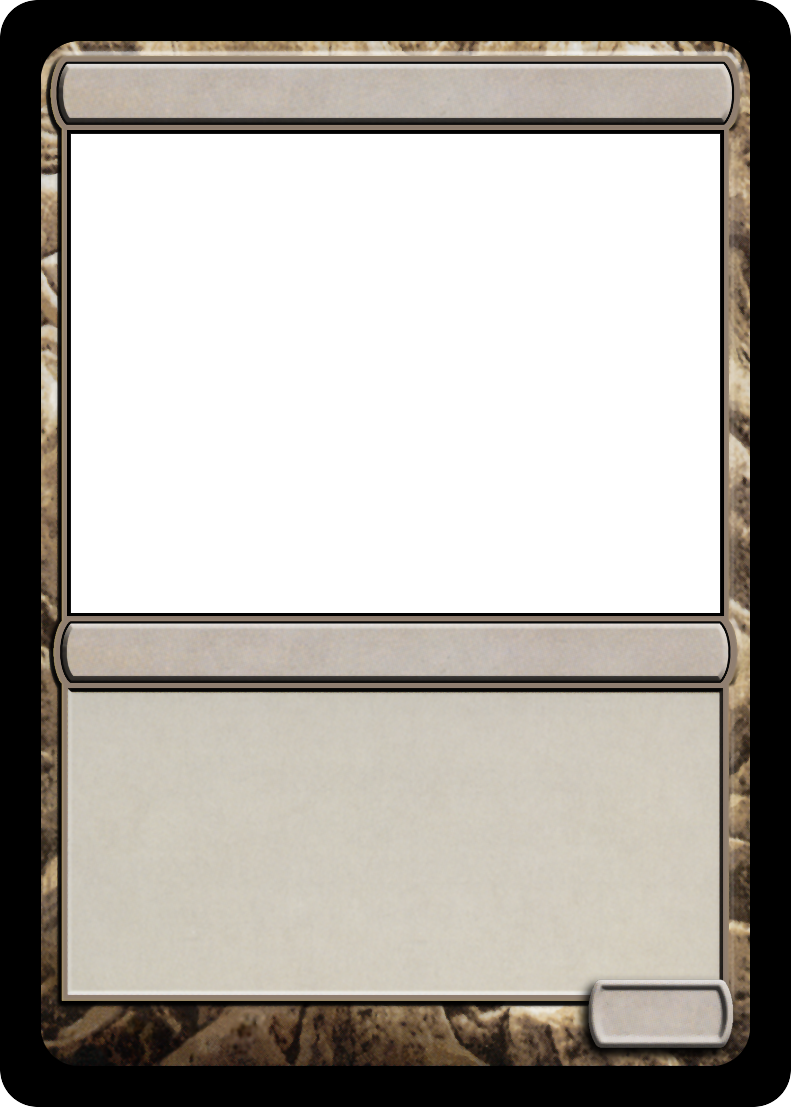
\includegraphics[width=\cardwidth cm, height=\cardheight cm]{fonds/fond_personnage.png}};

    %Titre
	\node[anchor=center] at (\titleX,\titleY) {\titlefont Philippe};

	%Image
	\node[anchor=center] at (\imageX,\imageY) {
\includegraphics[width=\imageWidth px, height=\imageHeight px]{images/philippe.png}};
	\node[anchor=center] at (6.1,4.5) {
\includegraphics[width=10 px, height=10 px]{fonds2/violet.jpg}};

	%Type
	\node[anchor=center] at (\typeX,\typeY) {\typefont Personnage Unique};

	%Description
	\node[anchor=north west, text width=5.6cm] (description) at (\descriptionX,\descriptionY) {\descriptionfont\setsize{6}(Mystérieux). Si vous êtes Philippe, posez cette carte devant vous au début de la partie. Personne ne peut prévoir vos plans et vous pouvez échanger votre personnage contre un autre laissé de côté après le tour de DSI. Vous avez le droit de porter une épée pendant la partie.\par};

	%Punchline
	\node[anchor=north west, text width=5.6cm, below = 1pt of description] (punchline) {\punchlinefont\setsize{5}{\bf "N'oubliez pas de remplir la feuille de choix pour le restaurant PEA. "}\par};

	%Separateur !!!!!PAS TOUCHE!!!!!
	\fill[black,path fading=west] (description.south west) rectangle (punchline.north);
	\fill[black,path fading=east] (punchline.north) rectangle (description.south east);

	%Numéro !!!!!PAS TOUCHE!!!!!
	\node[anchor=center] at (\numberX,\numberY) {\numberfont **/**};
\end{tikzpicture}\versoperso %Verso



%%%%%%%%%%%%%%%%%%%%%%%%%%%%%%%%%%%%%%%%%%%%%%%%%%%%%%%%%%%%%%
%%RENO
\begin{tikzpicture} %Recto
	%Fond
    \node[anchor=south west,inner sep=0] (carte) at (0,0) {
\includegraphics[width=7.1 cm, height=9.6 cm]{fonds/noir.png}};
    \node[anchor=center] at (carte.center) {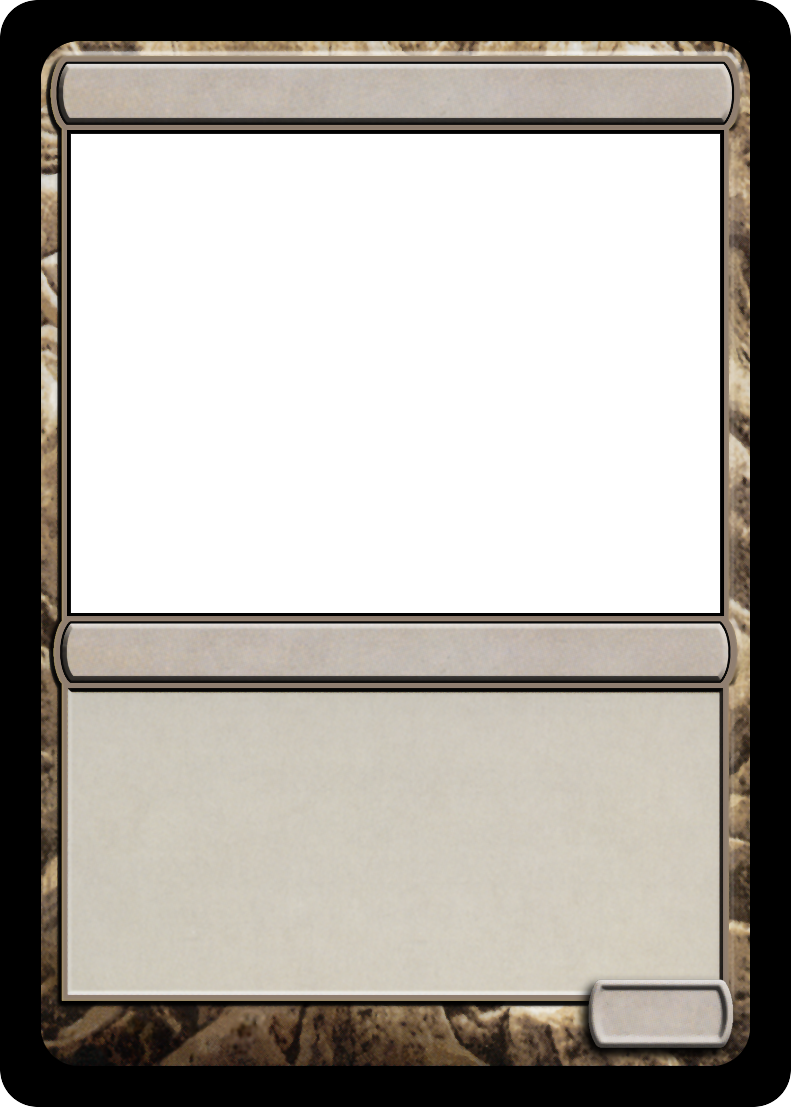
\includegraphics[width=\cardwidth cm, height=\cardheight cm]{fonds/fond_personnage.png}};

    %Titre
	\node[anchor=center] at (\titleX,\titleY) {\titlefont Reno};

	%Image
	\node[anchor=center] at (\imageX,\imageY) {
\includegraphics[width=\imageWidth px, height=\imageHeight px]{images/reno.jpg}};
	\node[anchor=center] at (6.1,4.5) {
\includegraphics[width=10 px, height=10 px]{fonds2/violet.jpg}};

	%Type
	\node[anchor=center] at (\typeX,\typeY) {\typefont Personnage Unique};

	%Description
	\node[anchor=north west, text width=5.6cm] (description) at (\descriptionX,\descriptionY) {\descriptionfont\setsize{6}(Parieur Colérique). Si vous êtes Renaud, posez cette carte devant vous au début de la partie. 
	Vous pouvez tapez très fort du doigt sur la table pour échanger une carte de votre main contre une carte malus ou { pari: pain au chocolat} de la défausse.\par};

	%Punchline
	\node[anchor=north west, text width=5.6cm, below = 1pt of description] (punchline) {\punchlinefont\setsize{5}{\bf "NON, JE NE SUIS PAS D'ACCORD!" ou "Je parie un pain au chocolat que je gagne mon prochain pari."}\par};

	%Separateur !!!!!PAS TOUCHE!!!!!
	\fill[black,path fading=west] (description.south west) rectangle (punchline.north);
	\fill[black,path fading=east] (punchline.north) rectangle (description.south east);

	%Numéro !!!!!PAS TOUCHE!!!!!
	\node[anchor=center] at (\numberX,\numberY) {\numberfont **/**};
\end{tikzpicture}\versoperso %Verso



%%%%%%%%%%%%%%%%%%%%%%%%%%%%%%%%%%%%%%%%%%%%%%%%%%%%%%%%%%%%%%
%%OBI
\begin{tikzpicture} %Recto
	%Fond
    \node[anchor=south west,inner sep=0] (carte) at (0,0) {
\includegraphics[width=7.1 cm, height=9.6 cm]{fonds/noir.png}};
    \node[anchor=center] at (carte.center) {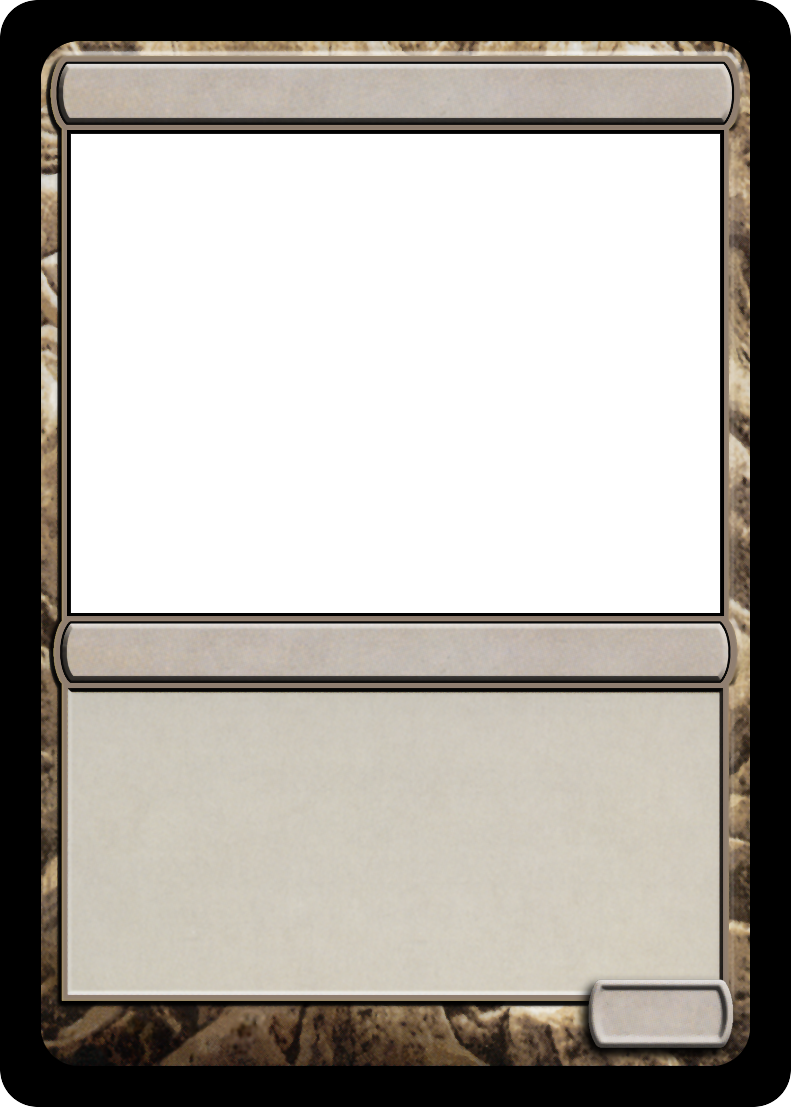
\includegraphics[width=\cardwidth cm, height=\cardheight cm]{fonds/fond_personnage.png}};

    %Titre
	\node[anchor=center] at (\titleX,\titleY) {\titlefont Olivier};

	%Image
	\node[anchor=center] at (\imageX,\imageY) {
\includegraphics[width=\imageWidth px, height=\imageHeight px]{images/obi.jpg}};
	\node[anchor=center] at (6.1,4.5) {
\includegraphics[width=10 px, height=10 px]{fonds2/violet.jpg}};

	%Type
	\node[anchor=center] at (\typeX,\typeY) {\typefont Personnage Unique};

	%Description
	\node[anchor=north west, text width=5.6cm] (description) at (\descriptionX,\descriptionY) {\descriptionfont\setsize{6}(Perfectionniste). Si vous êtes Olivier, posez cette carte devant vous au début de la partie. 
	Vous pouvez échanger votre bonus de tour pour choisir la valeur plutôt que celle révélée la prochaine fois qu'une révélation de carte est nécessaire durant votre tour.\par};

	%Punchline
	\node[anchor=north west, text width=5.6cm, below = 1pt of description] (punchline) {\punchlinefont\setsize{5}{\bf "Ce n'est pas de la surqualité. Je sais juste bosser correctement."}\par};

	%Separateur !!!!!PAS TOUCHE!!!!!
	\fill[black,path fading=west] (description.south west) rectangle (punchline.north);
	\fill[black,path fading=east] (punchline.north) rectangle (description.south east);

	%Numéro !!!!!PAS TOUCHE!!!!!
	\node[anchor=center] at (\numberX,\numberY) {\numberfont **/**};
\end{tikzpicture}\versoperso %Verso



%%%%%%%%%%%%%%%%%%%%%%%%%%%%%%%%%%%%%%%%%%%%%%%%%%%%%%%%%%%%%%
%%SYLVAin
\begin{tikzpicture} %Recto
	%Fond
    \node[anchor=south west,inner sep=0] (carte) at (0,0) {
\includegraphics[width=7.1 cm, height=9.6 cm]{fonds/noir.png}};
    \node[anchor=center] at (carte.center) {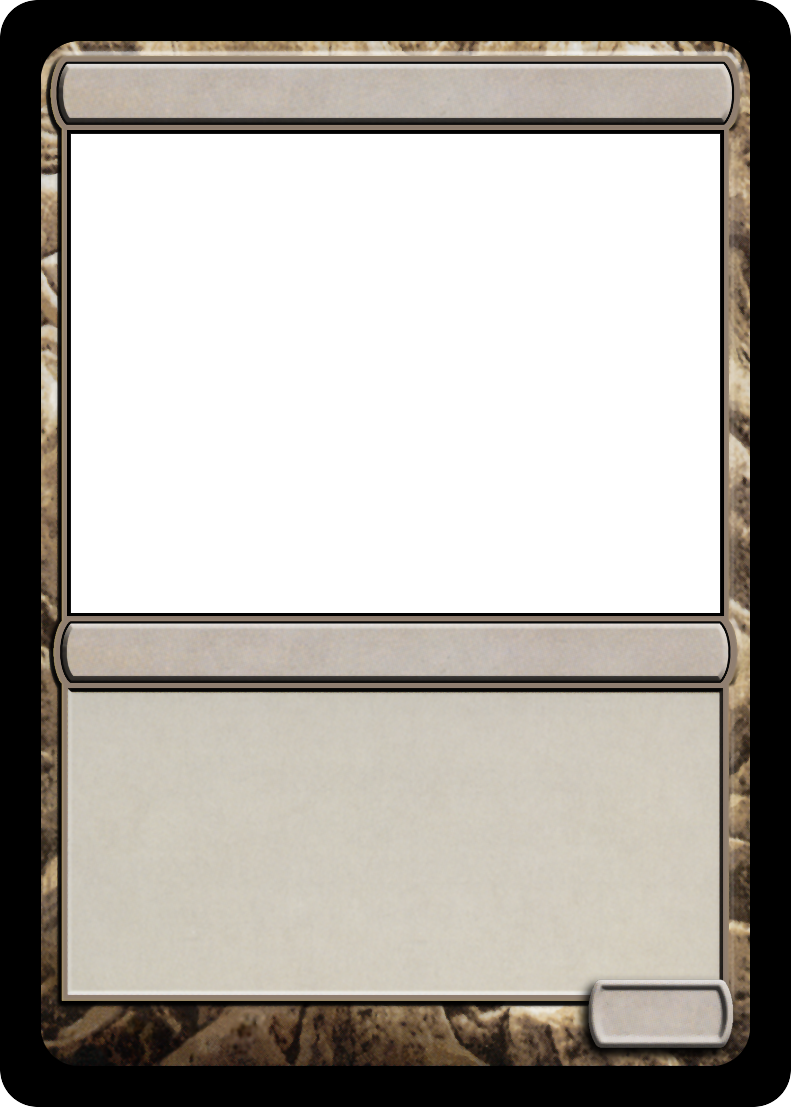
\includegraphics[width=\cardwidth cm, height=\cardheight cm]{fonds/fond_personnage.png}};

    %Titre
	\node[anchor=center] at (\titleX,\titleY) {\titlefont Sylvain};

	%Image
	\node[anchor=center] at (\imageX,\imageY) {
\includegraphics[width=\imageWidth px, height=\imageHeight px]{images/sylvain.jpg}};
	\node[anchor=center] at (6.1,4.5) {
\includegraphics[width=10 px, height=10 px]{fonds2/violet.jpg}};

	%Type
	\node[anchor=center] at (\typeX,\typeY) {\typefont Personnage Unique};

	%Description
	\node[anchor=north west, text width=5.6cm] (description) at (\descriptionX,\descriptionY) {\descriptionfont\setsize{6}(Rancunier). Lorsque qu'un joueur joue une carte défavorable contre vous, vous pouvez le nommer cet imprudent comme votre nouvel ennemi numéro 1 à abattre. Vous doublez les cartes malus que vous appliquez à votre ennemi. \par};

	%Punchline
	\node[anchor=north west, text width=5.6cm, below = 1pt of description] (punchline) {\punchlinefont\setsize{5}{\bf "Il a bafoué les règles de la chevalerie. Je lui ferai manger ses parents en chili con carne. Ou payer des croissants."}\par};

	%Separateur !!!!!PAS TOUCHE!!!!!
	\fill[black,path fading=west] (description.south west) rectangle (punchline.north);
	\fill[black,path fading=east] (punchline.north) rectangle (description.south east);

	%Numéro !!!!!PAS TOUCHE!!!!!
	\node[anchor=center] at (\numberX,\numberY) {\numberfont **/**};
\end{tikzpicture}\versoperso %Verso


%%%%%%%%%%%%%%%%%%%%%%%%%%%%%%%%%%%%%%%%%%%%%%%%%%%%%%%%%%%%%%
%%Zoe
\begin{tikzpicture} %Recto
	%Fond
    \node[anchor=south west,inner sep=0] (carte) at (0,0) {
\includegraphics[width=7.1 cm, height=9.6 cm]{fonds/noir.png}};
    \node[anchor=center] at (carte.center) {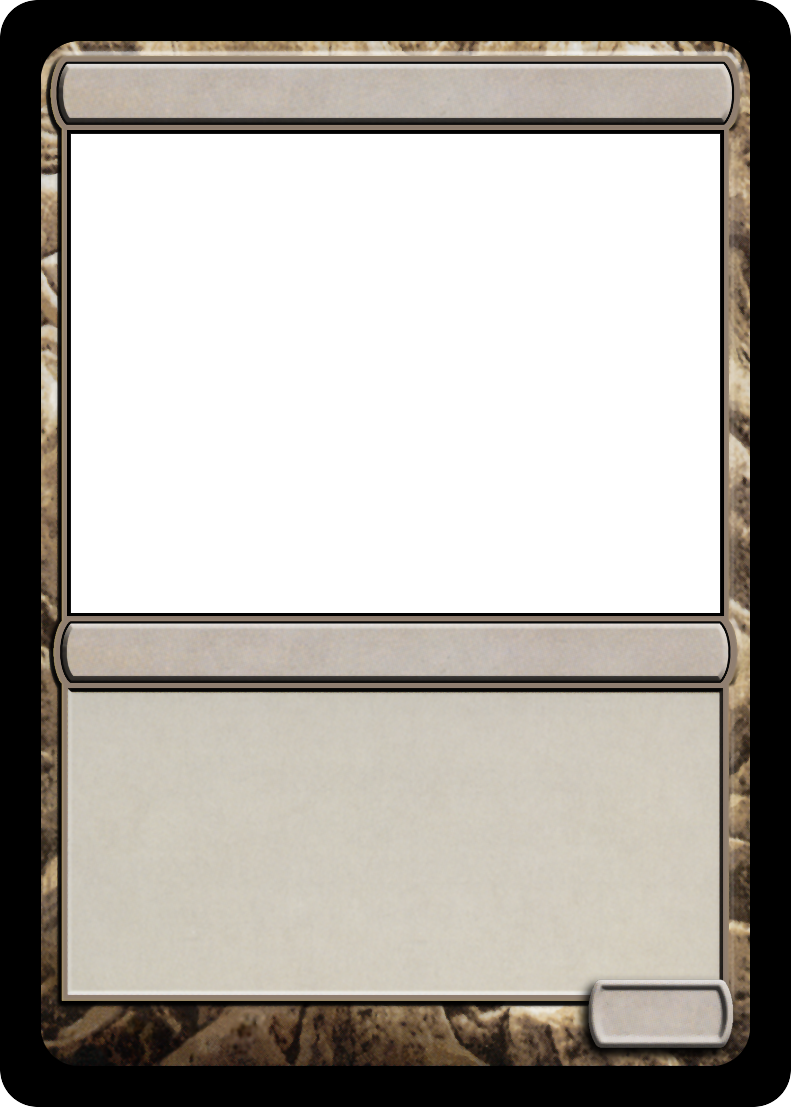
\includegraphics[width=\cardwidth cm, height=\cardheight cm]{fonds/fond_personnage.png}};

    %Titre
	\node[anchor=center] at (\titleX,\titleY) {\titlefont Zoé};

	%Image
	\node[anchor=center] at (\imageX,\imageY) {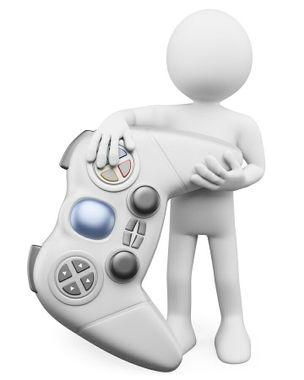
\includegraphics[width=\imageWidth px, height=\imageHeight px]{images/zoe.jpg}};
	\node[anchor=center] at (6.1,4.5) {
\includegraphics[width=10 px, height=10 px]{fonds2/violet.jpg}};

	%Type
	\node[anchor=center] at (\typeX,\typeY) {\typefont Personnage Unique};

	%Description
	\node[anchor=north west, text width=5.6cm] (description) at (\descriptionX,\descriptionY) {\descriptionfont\setsize{6}(Gameuse)  Vous voyez très bien ce qui est God Tier totalement OP ou trash Tier et vous pouvez donc nerf/buff de 1 la valeur d'une carte révélée pendant votre tour. Vous avez compris le sens de cette phrase sans qu'on vous l'explique et l'expliquez aux autres joueurs un peu boomer. \par};

	%Punchline
	\node[anchor=north west, text width=5.6cm, below = 1pt of description] (punchline) {\punchlinefont\setsize{5}{\bf "Je suis biclassée Magot niveau 27/Cryptologue niveau 12."}\par};

	%Separateur !!!!!PAS TOUCHE!!!!!
	\fill[black,path fading=west] (description.south west) rectangle (punchline.north);
	\fill[black,path fading=east] (punchline.north) rectangle (description.south east);

	%Numéro !!!!!PAS TOUCHE!!!!!
	\node[anchor=center] at (\numberX,\numberY) {\numberfont **/**};
\end{tikzpicture}\versoperso %Verso


%%%%%%%%%%%%%%%%%%%%%%%%%%%%%%%%%%%%%%%%%%%%%%%%%%%%%%%%%%%%%%
%%David
\begin{tikzpicture} %Recto
	%Fond
    \node[anchor=south west,inner sep=0] (carte) at (0,0) {
\includegraphics[width=7.1 cm, height=9.6 cm]{fonds/noir.png}};
    \node[anchor=center] at (carte.center) {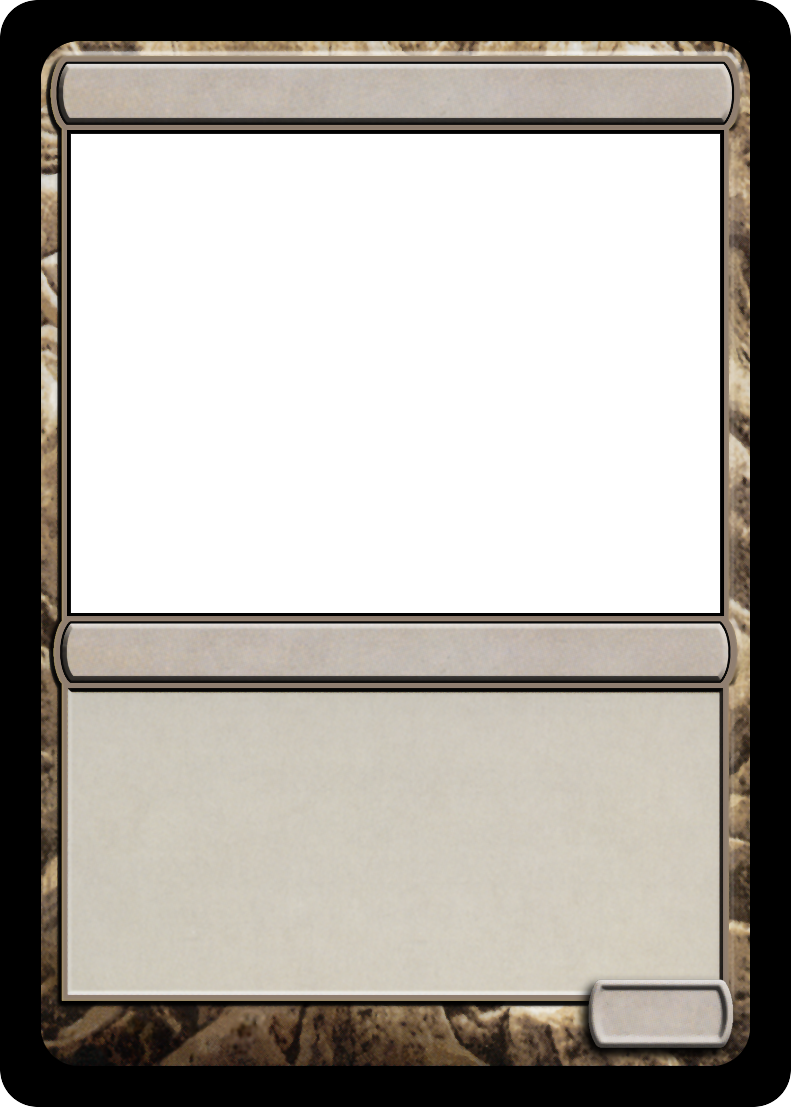
\includegraphics[width=\cardwidth cm, height=\cardheight cm]{fonds/fond_personnage.png}};

    %Titre
	\node[anchor=center] at (\titleX,\titleY) {\titlefont David};

	%Image
	\node[anchor=center] at (\imageX,\imageY) {
\includegraphics[width=\imageWidth px, height=\imageHeight px]{images/david.jpg}};
	\node[anchor=center] at (6.1,4.5) {
\includegraphics[width=10 px, height=10 px]{fonds2/violet.jpg}};

	%Type
	\node[anchor=center] at (\typeX,\typeY) {\typefont Personnage Unique};

	%Description
	\node[anchor=north west, text width=5.6cm] (description) at (\descriptionX,\descriptionY) {\descriptionfont\setsize{6}(Sportif) Si la carte Lucie d'Ecosse ou Challenge sportif est dans la défausse, vous avez le droit de défaussez une carte au début de votre tour au lieu de travailler.  Vous avez le droit de charier les autres joueurs, d'esquiver les coups de pieds, raconter la blague des prêtres et de maudire votre  insupportable collègue de bureau.\par};

	%Punchline
	\node[anchor=north west, text width=5.6cm, below = 1pt of description] (punchline) {\punchlinefont\setsize{5}{\bf "Ah, et un détail de  plus : vous n'avez pas de prépuce."}\par};

	%Separateur !!!!!PAS TOUCHE!!!!!
	\fill[black,path fading=west] (description.south west) rectangle (punchline.north);
	\fill[black,path fading=east] (punchline.north) rectangle (description.south east);

	%Numéro !!!!!PAS TOUCHE!!!!!
	\node[anchor=center] at (\numberX,\numberY) {\numberfont **/**};
\end{tikzpicture}\versoperso %Verso


%%%%%%%%%%%%%%%%%%%%%%%%%%%%%%%%%%%%%%%%%%%%%%%%%%%%%%%%%%%%%%
%%Thomas
\begin{tikzpicture} %Recto
	%Fond
    \node[anchor=south west,inner sep=0] (carte) at (0,0) {
\includegraphics[width=7.1 cm, height=9.6 cm]{fonds/noir.png}};
    \node[anchor=center] at (carte.center) {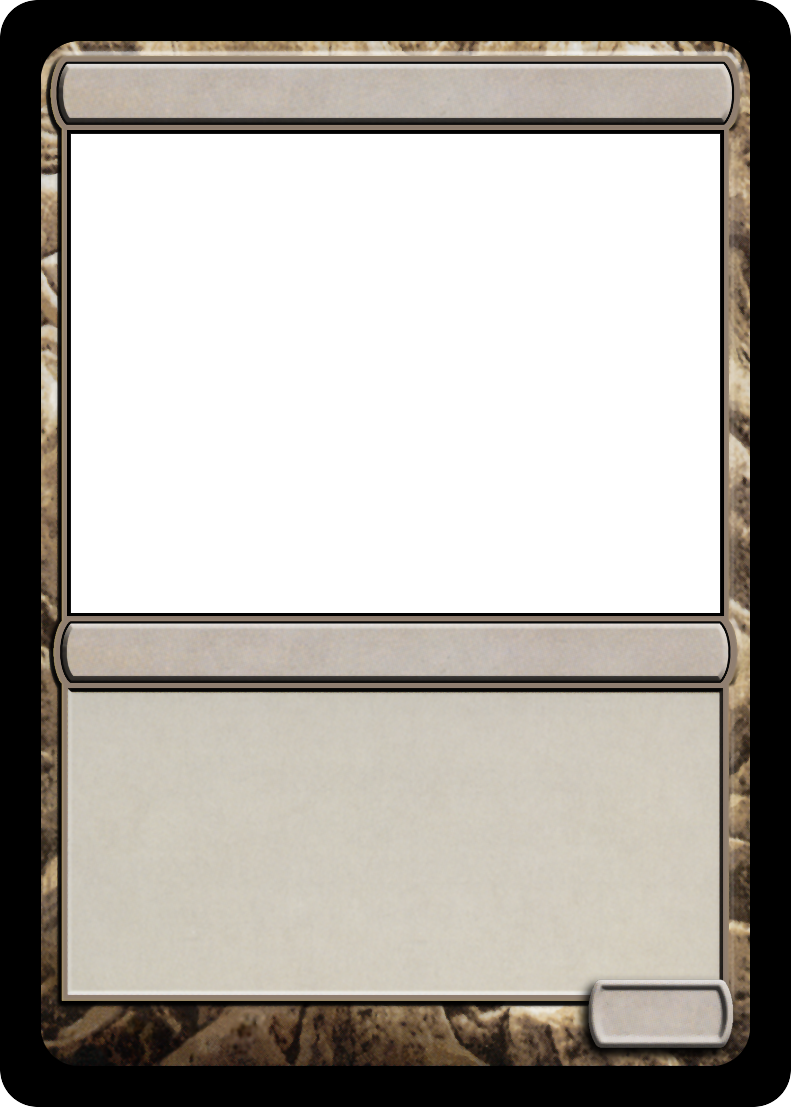
\includegraphics[width=\cardwidth cm, height=\cardheight cm]{fonds/fond_personnage.png}};

    %Titre
	\node[anchor=center] at (\titleX,\titleY) {\titlefont Thomas};

	%Image
	\node[anchor=center] at (\imageX,\imageY) {
\includegraphics[width=\imageWidth px, height=\imageHeight px]{images/thomas.jpg}};
	\node[anchor=center] at (6.1,4.5) {
\includegraphics[width=10 px, height=10 px]{fonds2/violet.jpg}};

	%Type
	\node[anchor=center] at (\typeX,\typeY) {\typefont Personnage Unique};

	%Description
	\node[anchor=north west, text width=5.6cm] (description) at (\descriptionX,\descriptionY) {\descriptionfont\setsize{6}(L'élu.) Vous êtes celui qui ramènera l'équilibre dans la crypto. Au début de votre tour, vous pouvez aller chercher l'apocalypse quantique dans la défausse ou le tas et la donner à un autre joueur pour promouvoir la crypto     post quantique. Dans ce cas, vous pouvez jouer un tour supplémentaire en tant que PQ-cryptologue après votre tour. \par};

	%Punchline
	\node[anchor=north west, text width=5.6cm, below = 1pt of description] (punchline) {\punchlinefont\setsize{6}{\bf "Le modèle du groupe générique  c'est pourri."}\par};

	%Separateur !!!!!PAS TOUCHE!!!!!
	\fill[black,path fading=west] (description.south west) rectangle (punchline.north);
	\fill[black,path fading=east] (punchline.north) rectangle (description.south east);

	%Numéro !!!!!PAS TOUCHE!!!!!
	\node[anchor=center] at (\numberX,\numberY) {\numberfont **/**};
\end{tikzpicture}\versoperso %Verso


%%%%%%%%%%%%%%%%%%%%%%%%%%%%%%%%%%%%%%%%%%%%%%%%%%%%%%%%%%%%%%
%%Aurélien
\begin{tikzpicture} %Recto
	%Fond
    \node[anchor=south west,inner sep=0] (carte) at (0,0) {
\includegraphics[width=7.1 cm, height=9.6 cm]{fonds/noir.png}};
    \node[anchor=center] at (carte.center) {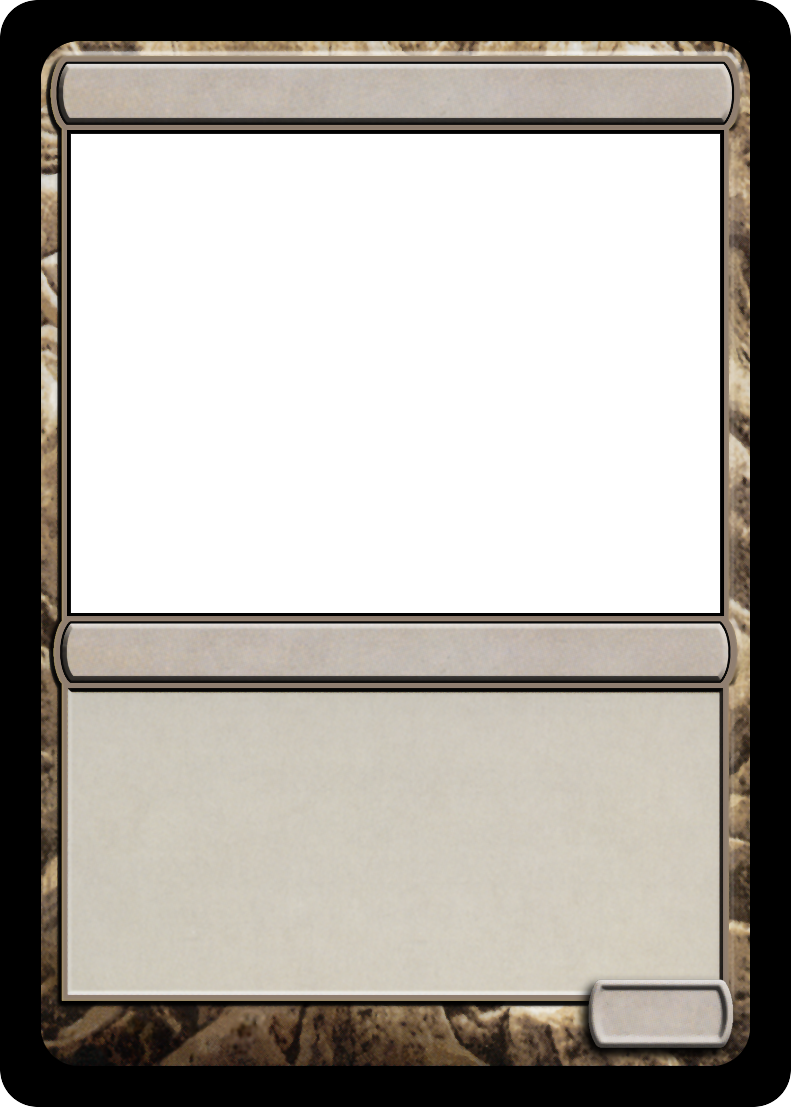
\includegraphics[width=\cardwidth cm, height=\cardheight cm]{fonds/fond_personnage.png}};

    %Titre
	\node[anchor=center] at (\titleX,\titleY) {\titlefont Aurélien};

	%Image
	\node[anchor=center] at (\imageX,\imageY) {
\includegraphics[width=\imageWidth px, height=\imageHeight px]{images/Aurelien.jpg}};
	\node[anchor=center] at (6.1,4.5) {
\includegraphics[width=10 px, height=10 px]{fonds2/violet.jpg}};

	%Type
	\node[anchor=center] at (\typeX,\typeY) {\typefont Personnage Unique};

	%Description
	\node[anchor=north west, text width=5.6cm] (description) at (\descriptionX,\descriptionY) {\descriptionfont\setsize{6}(Affamé) Votre appétit vorace vous permet de prendre une carte du dessus du tas à manger dans votre main, puis de digérer une carte de votre main vers la défausse. Les joueurs en retard se font copieusement insulter. Vous pouvez échanger toute carte liée à la nourriture dans la défausse contre une carte de votre main.\par};

	%Punchline
	\node[anchor=north west, text width=5.6cm, below = 1pt of description] (punchline) {\punchlinefont\setsize{6}{\bf "Bon, c'est l'heure !!!."}\par};

	%Separateur !!!!!PAS TOUCHE!!!!!
	\fill[black,path fading=west] (description.south west) rectangle (punchline.north);
	\fill[black,path fading=east] (punchline.north) rectangle (description.south east);

	%Numéro !!!!!PAS TOUCHE!!!!!
	\node[anchor=center] at (\numberX,\numberY) {\numberfont **/**};
\end{tikzpicture}\versoperso %Verso


















%%%%%%%%%%%%%%%%%%%%%%%%%%%%%%%%%%%%%%%%%%%%%%%%%%%%%%%%%%%%%% PMO
\begin{tikzpicture} %Recto
	%Fond
    \node[anchor=south west,inner sep=0] (carte) at (0,0) {
\includegraphics[width=7.1 cm, height=9.6 cm]{fonds/noir.png}};
    \node[anchor=center] at (carte.center) {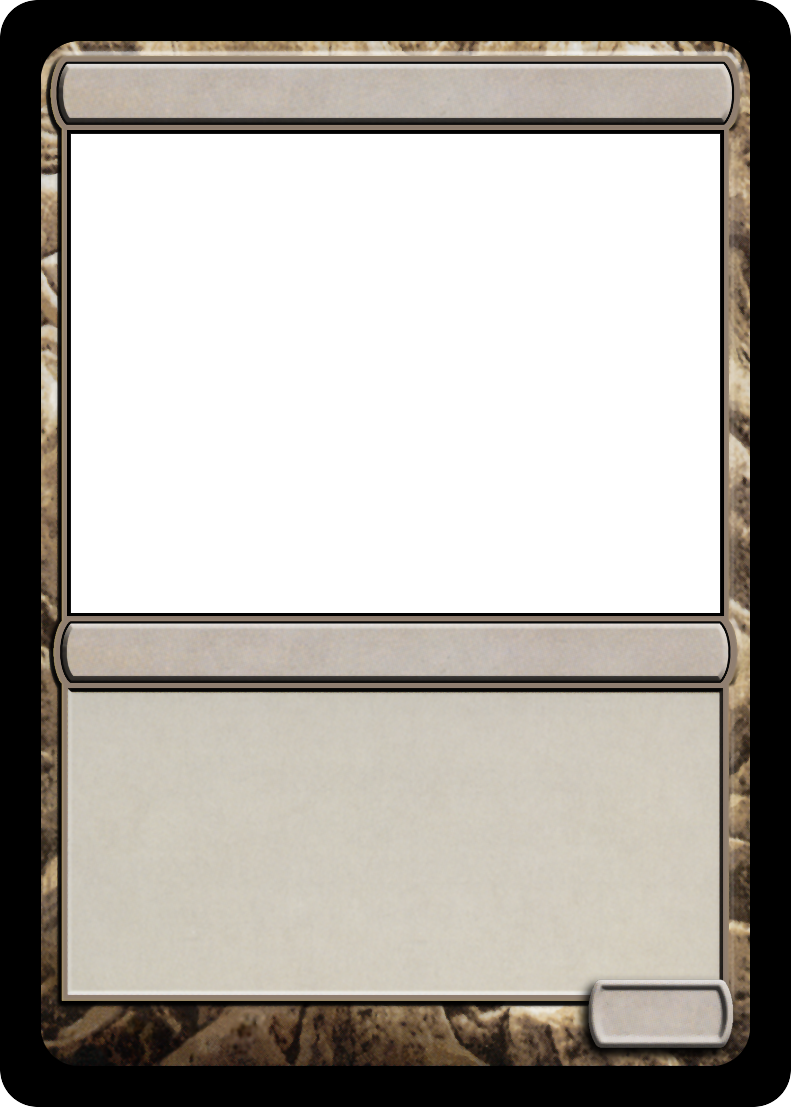
\includegraphics[width=\cardwidth cm, height=\cardheight cm]{fonds/fond_personnage.png}};

    %Titre
	\node[anchor=center] at (\titleX,\titleY) {\titlefont Prestataire};

	%Image
	\node[anchor=center] at (\imageX,\imageY) {
\includegraphics[width=\imageWidth px, height=\imageHeight px]{images/presta.jpg}};
	\node[anchor=center] at (6.1,4.5) {
\includegraphics[width=10 px, height=10 px]{fonds2/violet.jpg}};

	%Type
	\node[anchor=center] at (\typeX,\typeY) {\typefont Personnage Additionnel};

	%Description
	\node[anchor=north west, text width=5.6cm] (description) at (\descriptionX,\descriptionY) {\descriptionfont\setsize{6}(Mission)Vous effectuez une mission de remplacement d'un joueur. Choisissez un rôle et jouez à la place de ce joueur. S'il ne devait pas jouer, vous n'avez pas de contrat et passez votre tour.\par
(Esclave) Tout le monde sauf le stagiaire peut vous demander d'apporter un café.\par};

	
	%Punchline
	\node[anchor=north west, text width=5.6cm, below = 1pt of description] (punchline) {\punchlinefont\setsize{6} Si vous trouvez votre poste pourri, dites vous qu'il reste les prestas.\par};

	%Separateur !!!!!PAS TOUCHE!!!!!
	\fill[black,path fading=west] (description.south west) rectangle (punchline.north);
	\fill[black,path fading=east] (punchline.north) rectangle (description.south east);

	%Numéro !!!!!PAS TOUCHE!!!!!
	\node[anchor=center] at (\numberX,\numberY) {\numberfont 1/9};
\end{tikzpicture}\versoperso %Verso

%%%%%%%%%%%%%%%%%%%%%%%%%%%%%%%%%%%%%%%%%%%%%%%%%%%%%%%%%%%%%% PMO
\begin{tikzpicture} %Recto
	%Fond
    \node[anchor=south west,inner sep=0] (carte) at (0,0) {
\includegraphics[width=7.1 cm, height=9.6 cm]{fonds/noir.png}};
    \node[anchor=center] at (carte.center) {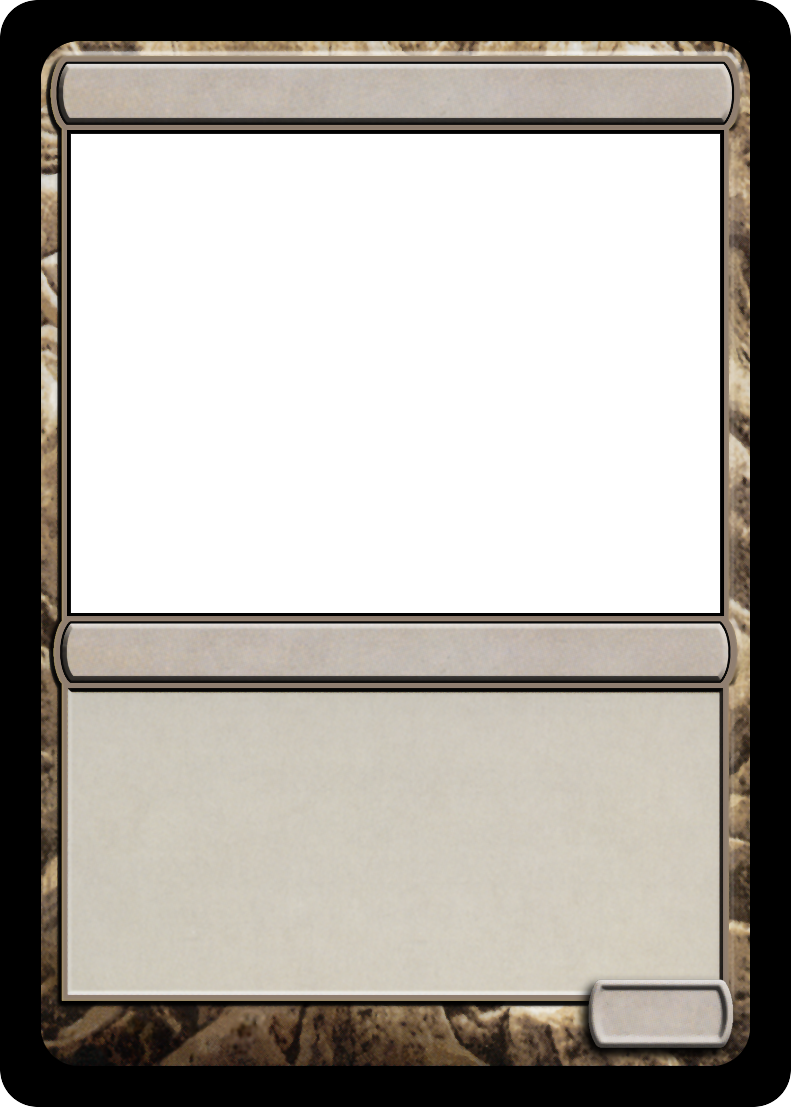
\includegraphics[width=\cardwidth cm, height=\cardheight cm]{fonds/fond_personnage.png}};

    %Titre
	\node[anchor=center] at (\titleX,\titleY) {\titlefont Gestionnaire de Conf};

	%Image
	\node[anchor=center] at (\imageX,\imageY) {\includegraphics[width=\imageWidth px, height=\imageHeight px]{images/P2_necro.png}};
\node[anchor=center] at (6.1,4.5) {\includegraphics[width=10 px, height=10 px]{fonds2/antiviolet.jpg}};

	%Type
	\node[anchor=center] at (\typeX,\typeY) {\typefont Personnage Additionnel};

	%Description
	\node[anchor=north west, text width=5.6cm] (description) at (\descriptionX,\descriptionY) {\descriptionfont\setsize{8}(Nécromancie) Vous êtes responsable de la défausse pour ce tour et la gardez près de vous. Vous pouvez échanger une carte de votre main contre une carte de la défausse avec la même valeur.\par};

	
	%Punchline
	\node[anchor=north west, text width=5.6cm, below = 1pt of description] (punchline) {\punchlinefont\setsize{8} Je n’ai ni UO ni CBB,  mais ce que j’ai, je te le donne : Au nom de Chorus2, Git et SVN : Lève-toi et marche.\par};

	%Separateur !!!!!PAS TOUCHE!!!!!
	\fill[black,path fading=west] (description.south west) rectangle (punchline.north);
	\fill[black,path fading=east] (punchline.north) rectangle (description.south east);

	%Numéro !!!!!PAS TOUCHE!!!!!
	\node[anchor=center] at (\numberX,\numberY) {\numberfont 2/9};
\end{tikzpicture}\versoperso %Verso

%%%%%%%%%%%%%%%%%%%%%%%%%%%%%%%%%%%%%%%%%%%%%%%%%%%%%%%%%%%%%% PMO
\begin{tikzpicture} %Recto
	%Fond
    \node[anchor=south west,inner sep=0] (carte) at (0,0) {\includegraphics[width=7.1 cm, height=9.6 cm]{fonds/noir.png}};
    \node[anchor=center] at (carte.center) {\includegraphics[width=\cardwidth cm, height=\cardheight cm]{fonds/fond_personnage.png}};

    %Titre
	\node[anchor=center] at (\titleX,\titleY) {\titlefont Ponte N++};

	%Image
	\node[anchor=center] at (\imageX,\imageY) {\includegraphics[width=\imageWidth px, height=\imageHeight px]{images/ponte.jpg}};
\node[anchor=center] at (6.1,4.5) {\includegraphics[width=10 px, height=10 px]{fonds2/violet.jpg}};

	%Type
	\node[anchor=center] at (\typeX,\typeY) {\typefont Personnage Additionnel};

	%Description
	\node[anchor=north west, text width=5.6cm] (description) at (\descriptionX,\descriptionY) {\descriptionfont\setsize{7}(Tyrannie) Chaque fois qu'un joueur joue une carte qui cible un autre joueur VOUS décidez à qui l'effet s'applique.\par
	(Passé technique lointain) VOUS ne pouvez jouer aucune carte contenant un mot qu'un enfant de huit ans ne connaît pas.\par};

	
	%Punchline
	\node[anchor=north west, text width=5.6cm, below = 1pt of description] (punchline) {\punchlinefont\setsize{6}(Permanent)Tout le monde est obséquieux avec VOUS pendant ce tour.\par};

	%Separateur !!!!!PAS TOUCHE!!!!!
	\fill[black,path fading=west] (description.south west) rectangle (punchline.north);
	\fill[black,path fading=east] (punchline.north) rectangle (description.south east);

	%Numéro !!!!!PAS TOUCHE!!!!!
	\node[anchor=center] at (\numberX,\numberY) {\numberfont 3/9};
\end{tikzpicture}\versoperso %Verso

%%%%%%%%%%%%%%%%%%%%%%%%%%%%%%%%%%%%%%%%%%%%%%%%%%%%%%%%%%%%%% PMO
\begin{tikzpicture} %Recto
	%Fond
    \node[anchor=south west,inner sep=0] (carte) at (0,0) {\includegraphics[width=7.1 cm, height=9.6 cm]{fonds/noir.png}};
    \node[anchor=center] at (carte.center) {\includegraphics[width=\cardwidth cm, height=\cardheight cm]{fonds/fond_personnage.png}};

    %Titre
	\node[anchor=center] at (\titleX,\titleY) {\titlefont Commercial};

	%Image
	\node[anchor=center] at (\imageX,\imageY) {\includegraphics[width=\imageWidth px, height=\imageHeight px]{images/market2.jpg}};
\node[anchor=center] at (6.1,4.5) {\includegraphics[width=10 px, height=10 px]{fonds2/violet.jpg}};

	%Type
	\node[anchor=center] at (\typeX,\typeY) {\typefont Personnage Additionnel};

	%Description
	\node[anchor=north west, text width=5.6cm] (description) at (\descriptionX,\descriptionY) {\descriptionfont\setsize{6}(Deal fructueux) Le commercial peut regarder la main d'un joueur et jouer immédiatement une carte s'y trouvant en plus de ses actions, ou bien échanger des cartes de sa main contre un nombre identique de cartes du haut du tas.\par};

	%Punchline
	\node[anchor=north west, text width=5.6cm, below = 1pt of description] (punchline) {\punchlinefont\setsize{6}(Un peu lent) Si une carte contient un terme technique, faites répéter le joueur et dites que vous le saviez.\par};

	%Separateur !!!!!PAS TOUCHE!!!!!
	\fill[black,path fading=west] (description.south west) rectangle (punchline.north);
	\fill[black,path fading=east] (punchline.north) rectangle (description.south east);

	%Numéro !!!!!PAS TOUCHE!!!!!
	\node[anchor=center] at (\numberX,\numberY) {\numberfont 4/9};
\end{tikzpicture}\versoperso %Verso

%%%%%%%%%%%%%%%%%%%%%%%%%%%%%%%%%%%%%%%%%%%%%%%%%%%%%%%%%%%%%% PMO
\begin{tikzpicture} %Recto
	%Fond
    \node[anchor=south west,inner sep=0] (carte) at (0,0) {\includegraphics[width=7.1 cm, height=9.6 cm]{fonds/noir.png}};
    \node[anchor=center] at (carte.center) {\includegraphics[width=\cardwidth cm, height=\cardheight cm]{fonds/fond_personnage.png}};

    %Titre
	\node[anchor=center] at (\titleX,\titleY) {\titlefont WPM (Projet Manager Grouillot)};

	%Image
	\node[anchor=center] at (\imageX,\imageY) {\includegraphics[width=\imageWidth px, height=\imageHeight px]{images/P5_wpm.jpg}};
\node[anchor=center] at (6.1,4.5) {\includegraphics[width=10 px, height=10 px]{fonds2/violet.jpg}};

	%Type
	\node[anchor=center] at (\typeX,\typeY) {\typefont Personnage Additionnel};

	%Description
	\node[anchor=north west, text width=5.6cm] (description) at (\descriptionX,\descriptionY) {\descriptionfont\setsize{6}(Planification transverse) Le WPM prend la carte planning puis révèle une carte du tas. Si elle est supérieure à 3,  il peut le donne au joueur de son choix en échange d'un permanent vert devant lui ou d'une carte bonus de la défausse. Placez le permanent devant le WPM comme s'il venait de le jouer.\par};

	%Punchline
	\node[anchor=north west, text width=5.6cm, below = 1pt of description] (punchline) {\punchlinefont\setsize{6}(Permanent) Dès que vous êtes concentré, un joueur peut vous demander un numéro d'OS.\par};

	%Separateur !!!!!PAS TOUCHE!!!!!
	\fill[black,path fading=west] (description.south west) rectangle (punchline.north);
	\fill[black,path fading=east] (punchline.north) rectangle (description.south east);

	%Numéro !!!!!PAS TOUCHE!!!!!
	\node[anchor=center] at (\numberX,\numberY) {\numberfont 5/9};
\end{tikzpicture}\versoperso %Verso

%%%%%%%%%%%%%%%%%%%%%%%%%%%%%%%%%%%%%%%%%%%%%%%%%%%%%%%%%%%%%% DEVELOPPEUR
\begin{tikzpicture} %Recto
	%Fond
    \node[anchor=south west,inner sep=0] (carte) at (0,0) {\includegraphics[width=7.1 cm, height=9.6 cm]{fonds/noir.png}};
    \node[anchor=center] at (carte.center) {\includegraphics[width=\cardwidth cm, height=\cardheight cm]{fonds/fond_personnage.png}};

    %Titre
	\node[anchor=center] at (\titleX,\titleY) {\titlefont Développeur};

	%Image
	\node[anchor=center] at (\imageX,\imageY) {\includegraphics[width=\imageWidth px, height=\imageHeight px]{images/P6_Dev.jpg}};
\node[anchor=center] at (6.1,4.5) {\includegraphics[width=10 px, height=10 px]{fonds2/violet.jpg}};

	%Type
	\node[anchor=center] at (\typeX,\typeY) {\typefont Personnage Additionel};

	%Description
	\node[anchor=north west, text width=5.6cm] (description) at (\descriptionX,\descriptionY) {\descriptionfont\setsize{8}(Développement) Le développeur peut imputer une carte bonus supplémentaire.\par};

	%Punchline
	\node[anchor=north west, text width=5.6cm, below = 1pt of description] (punchline) {\punchlinefont\setsize{8}(Swag) Les joueurs de sexe opposé vous regardent avec méfiance pendant ce tour.\par};

	%Separateur !!!!!PAS TOUCHE!!!!!
	\fill[black,path fading=west] (description.south west) rectangle (punchline.north);
	\fill[black,path fading=east] (punchline.north) rectangle (description.south east);

	%Numéro !!!!!PAS TOUCHE!!!!!
	\node[anchor=center] at (\numberX,\numberY) {\numberfont 6/9};
\end{tikzpicture}\versoperso %Verso


%%%%%%%%%%%%%%%%%%%%%%%%%%%%
\begin{tikzpicture} %Recto
	%Fond
    \node[anchor=south west,inner sep=0] (carte) at (0,0) {\includegraphics[width=7.1 cm, height=9.6 cm]{fonds/noir.png}};
    \node[anchor=center] at (carte.center) {\includegraphics[width=\cardwidth cm, height=\cardheight cm]{fonds/fond_personnage.png}};

    %Titre
	\node[anchor=center] at (\titleX,\titleY) {\titlefont PQ-Cryptologue };

	%Image
	\node[anchor=center] at (\imageX,\imageY) {\includegraphics[width=\imageWidth px, height=\imageHeight px]{images/P10_compo.jpg}};
\node[anchor=center] at (6.1,4.5) {\includegraphics[width=10 px, height=10 px]{fonds2/violet.jpg}};

	%Type
	\node[anchor=center] at (\typeX,\typeY) {\typefont Personnage Additionnel };

	%Description
	\node[anchor=north west, text width=5.6cm] (description) at (\descriptionX,\descriptionY) {\descriptionfont\setsize{6}(Intrication quantique) Devinez la valeur (parité) du bit quantique puis mesurez la en révèlant de la carte du haut du tas. En cas de succès, vous pouvez  activer le pouvoir de cryptologue,
 ignorer tout effet de carte défavorable à ce tour, envoyer l'apocalypse quantique à la défausse.\par};. 

	%Punchline
	\node[anchor=north west, text width=5.6cm, below = 1pt of description] (punchline) {\punchlinefont\setsize{6}(Escroquerie au O(n)) Vous pouvez ignorer toutes les constantes de l'univers en les négligeant.\par};

	%Separateur !!!!!PAS TOUCHE!!!!!
	\fill[black,path fading=west] (description.south west) rectangle (punchline.north);
	\fill[black,path fading=east] (punchline.north) rectangle (description.south east);

	%Numéro !!!!!PAS TOUCHE!!!!!
	\node[anchor=center] at (\numberX,\numberY) {\numberfont 7/9};
\end{tikzpicture}\versoperso %Verso

%%%%%%%%%%%%%%%%%%%%%%%%%%%%%%%%%%%%%%%%%%%%%%%%%%%%%%%%%%%%%% 8: IS
\begin{tikzpicture} %Recto
	%Fond
    \node[anchor=south west,inner sep=0] (carte) at (0,0) {\includegraphics[width=7.1 cm, height=9.6 cm]{fonds/noir.png}};
    \node[anchor=center] at (carte.center) {\includegraphics[width=\cardwidth cm, height=\cardheight cm]{fonds/fond_personnage.png}};

    %Titre
	\node[anchor=center] at (\titleX,\titleY) {\titlefont Officier BCSC};

	%Image
	\node[anchor=center] at (\imageX,\imageY) {\includegraphics[width=\imageWidth px, height=\imageHeight px]{images/P8_BCSC.jpg}};
	\node[anchor=center] at (6.1,4.5) {\includegraphics[width=10 px, height=10 px]{fonds2/violet.jpg}};
	
	%Type
	\node[anchor=center] at (\typeX,\typeY) {\typefont Personnage Additionnel};

	%Description
	\node[anchor=north west, text width=5.6cm] (description) at (\descriptionX,\descriptionY) {\descriptionfont\setsize{6}(Procédurier) Au début de son tour, l'officier BCSC peut appliquer la procédure et tout ou partie des effets suivants : faire tourner d'un quart de tour inverse un permanent, trier la défausse dans l'ordre de son choix, échanger une carte de sa main contre un malus de la défausse, couper le tas.\par};

	%Punchline
	\node[anchor=north west, text width=5.6cm, below = 1pt of description] (punchline) {\punchlinefont\setsize{6}(Permanent)`` Il est 15h30, il va falloir revenir Lundi." .\par};

	%Separateur !!!!!PAS TOUCHE!!!!!
	\fill[black,path fading=west] (description.south west) rectangle (punchline.north);
	\fill[black,path fading=east] (punchline.north) rectangle (description.south east);

	%Numéro !!!!!PAS TOUCHE!!!!!
	\node[anchor=center] at (\numberX,\numberY) {\numberfont 8/9};
\end{tikzpicture}\versoperso %Verso

%%%%%%%%%%%%%%%%%%%%%%%%%%%%
\begin{tikzpicture} %Recto
	%Fond
    \node[anchor=south west,inner sep=0] (carte) at (0,0) {\includegraphics[width=7.1 cm, height=9.6 cm]{fonds/noir.png}};
    \node[anchor=center] at (carte.center) {\includegraphics[width=\cardwidth cm, height=\cardheight cm]{fonds/fond_personnage.png}};

    %Titre
	\node[anchor=center] at (\titleX,\titleY) {\titlefont RH };

	%Image
	\node[anchor=center] at (\imageX,\imageY) {\includegraphics[width=\imageWidth px, height=\imageHeight px]{images/perso_RH.jpg}};
	\node[anchor=center] at (6.1,4.5) {\includegraphics[width=10 px, height=10 px]{fonds2/violet.jpg}};

	%Type
	\node[anchor=center] at (\typeX,\typeY) {\typefont Personnage  Inutile };

	%Description
	\node[anchor=north west, text width=5.6cm] (description) at (\descriptionX,\descriptionY) {\descriptionfont\setsize{7}(Message important) La RH peut rejouer la carte neutre la plus au fond de la défausse au début de son tour.\par (Inutilité) Personne ne vous voit jamais. Par conséquent personne ne peut cibler la RH avec un effet. Hormis le choix de cible, tout les autres effets s'appliquent.\par};. 

	%Punchline
	\node[anchor=north west, text width=5.6cm, below = 1pt of description] (punchline) {\punchlinefont\setsize{6}\par`` Vivez votre aventure THALES (de**erdez-vous)."\par};

	
	%Separateur !!!!!PAS TOUCHE!!!!!
	\fill[black,path fading=west] (description.south west) rectangle (punchline.north);
	\fill[black,path fading=east] (punchline.north) rectangle (description.south east);

	%Numéro !!!!!PAS TOUCHE!!!!!
	\node[anchor=center] at (\numberX,\numberY) {\numberfont 9/9};
\end{tikzpicture}\versoperso %Verso

%--------------------------CARTES WIN CONDITION------------------------------------------------------------------------------------------------
\begin{tikzpicture} %Recto
	%Fond
    \node[anchor=south west,inner sep=0] (carte) at (0,0) {\includegraphics[width=7.1 cm, height=9.6 cm]{fonds/noir.png}};
    \node[anchor=center] at (carte.center) {\includegraphics[width=\cardwidth cm, height=\cardheight cm]{fonds/fond_anssi.png}};

    %Titre
	\node[anchor=center] at (\titleX,\titleY) {\titlefont CryptoText};

	%Image
	\node[anchor=center] at (\imageX,\imageY) {\includegraphics[width=\imageWidth px, height=\imageHeight px]{images/cryptotext.jpg}};
	\node[anchor=center] at (6.1,4.5) {\includegraphics[width=10 px, height=10 px]{fonds2/violet.jpg}};

	%Type
	\node[anchor=center] at (\typeX,\typeY) {\typefont Spécial (permanent)};

	%Description
	\node[anchor=north west, text width=5.6cm] (description) at (\descriptionX,\descriptionY) {\descriptionfont\setsize{6}Une opportunité dans une startup dynamique (et de ne plus jamais capitaliser ou imputer) vous sourit.
Vous ne pouvez jouer cette carte que si vous êtes le joueur avec le plus de cartes en main. Chaque fois que vous commencez un tour de jeu avec le plus de cartes, pivoter la carte (sens horaire). Au bout d'une rotation complète, vous gagnez la partie.
\par};
%Punchline
	\node[anchor=north west, text width=5.6cm, below = 1pt of description] (punchline) {\punchlinefont\setsize{6}Au revoir, au revoir président !!!.\par};
%Separateur !!!!!PAS TOUCHE!!!!!
	\fill[black,path fading=west] (description.south west) rectangle (punchline.north);
	\fill[black,path fading=east] (punchline.north) rectangle (description.south east);

	%Numéro !!!!!PAS TOUCHE!!!!!
	\node[anchor=center] at (\numberX,\numberY) {\numberfont \cardnumber};
\end{tikzpicture}\verso %Verso

%%%%%%%%%%%%%%%%%%%%%%%%%%%%
\begin{tikzpicture} %Recto
	%Fond
    \node[anchor=south west,inner sep=0] (carte) at (0,0) {\includegraphics[width=7.1 cm, height=9.6 cm]{fonds/noir.png}};
    \node[anchor=center] at (carte.center) {\includegraphics[width=\cardwidth cm, height=\cardheight cm]{fonds/fond_anssi.png}};

    %Titre
	\node[anchor=center] at (\titleX,\titleY) {\titlefont Crysalid};

	%Image
	\node[anchor=center] at (\imageX,\imageY) {\includegraphics[width=\imageWidth px, height=\imageHeight px]{images/crysalid.png}};
	\node[anchor=center] at (6.1,4.5) {\includegraphics[width=10 px, height=10 px]{fonds2/violet.jpg}};

	%Type
	\node[anchor=center] at (\typeX,\typeY) {\typefont Spécial (permanent)};

	%Description
	\node[anchor=north west, text width=5.6cm] (description) at (\descriptionX,\descriptionY) {\descriptionfont\setsize{8}Placez cette carte devant vous. Chaque fois que vous commencez un tour comme cryptologue ou développeur faites faire un quart de tour à cette carte pour compiler.
	Lorsque la carte a fait un tour complet, Crysalid compile sans erreur et vous remportez la partie. 
\par};
%Punchline
	\node[anchor=north west, text width=5.6cm, below = 1pt of description] (punchline) {\punchlinefont\setsize{8}Laissez-moi développer tranquille bordel !\par};
%Separateur !!!!!PAS TOUCHE!!!!!
	\fill[black,path fading=west] (description.south west) rectangle (punchline.north);
	\fill[black,path fading=east] (punchline.north) rectangle (description.south east);

	%Numéro !!!!!PAS TOUCHE!!!!!
	\node[anchor=center] at (\numberX,\numberY) {\numberfont \cardnumber};
\end{tikzpicture}\verso %Verso

%--------------------------CARTES NEUTRES------------------------------------------------------------------------------------------------


%%%%%%%%%%%%%%%%%%%%%%%%%%%%%%%%%%%%%%%%%%%%%%%%%%%%%%%%%%%%%%%%
\begin{tikzpicture} %Recto
	%Fond
    \node[anchor=south west,inner sep=0] (carte) at (0,0) {\includegraphics[width=7.1 cm, height=9.6 cm]{fonds/noir.png}};
    \node[anchor=center] at (carte.center) {\includegraphics[width=\cardwidth cm, height=\cardheight cm]{fonds/fond_neutre.png}};

    %Titre
	\node[anchor=center] at (\titleX,\titleY) {\titlefont Message de Framboise Vermeille};

	%Image
	\node[anchor=center] at (\imageX,\imageY) {\includegraphics[width=\imageWidth px, height=\imageHeight px]{images/Message.jpg}};
	\node[anchor=center] at (6.1,4.5) {\includegraphics[width=10 px, height=10 px]{fonds2/violet.jpg}};

	%Type
	\node[anchor=center] at (\typeX,\typeY) {\typefont Neutre};

	%Description
	\node[anchor=north west, text width=5.6cm] (description) at (\descriptionX,\descriptionY) {\descriptionfont\setsize{8}Tout le monde efface immédiatement le mail sans le lire. Mélangez la défausse dans le tas.\par};

	%Punchline
	\node[anchor=north west, text width=5.6cm, below = 1pt of description] (punchline) {\punchlinefont\setsize{8}``Chaque jour une vidéo. Vous n'avez pas pu assister à la première diffusion ? Vous pourrez vous en moquer autant aujourd'hui qu'hier en vous rendant sur la chaîne \color{blue}{BullshITS-TV} ! ''\par};

	%Separateur !!!!!PAS TOUCHE!!!!!
	\fill[black,path fading=west] (description.south west) rectangle (punchline.north);
	\fill[black,path fading=east] (punchline.north) rectangle (description.south east);

	%Numéro !!!!!PAS TOUCHE!!!!!
	\node[anchor=center] at (\numberX,\numberY) {\numberfont \cardnumber};
\end{tikzpicture}\verso %Verso


%%%%%%%%%%%%%%%%%%%%%%%%%%%%%%%%%%%%%%%%%%%%%%%%%%%%%%%%%%%%%%%%
\begin{tikzpicture} %Recto
	%Fond
    \node[anchor=south west,inner sep=0] (carte) at (0,0) {\includegraphics[width=7.1 cm, height=9.6 cm]{fonds/noir.png}};
    \node[anchor=center] at (carte.center) {\includegraphics[width=\cardwidth cm, height=\cardheight cm]{fonds/fond_neutre.png}};

    %Titre
	\node[anchor=center] at (\titleX,\titleY) {\titlefont Surcharge};

	%Image
	\node[anchor=center] at (\imageX,\imageY) {\includegraphics[width=\imageWidth px, height=\imageHeight px]{images/UO_Add1_surcharge.jpg}};
	\node[anchor=center] at (6.1,4.5) {\includegraphics[width=10 px, height=10 px]{fonds2/violet.jpg}};

	%Type
	\node[anchor=center] at (\typeX,\typeY) {\typefont Neutre (Permanent)};

	%Description
	\node[anchor=north west, text width=5.6cm] (description) at (\descriptionX,\descriptionY) {\descriptionfont\setsize{8}Posez cette carte devant vous. Tous les joueurs piochent deux cartes au lieu d'une au début de leur tour.\par};

	%Punchline
	\node[anchor=north west, text width=5.6cm, below = 1pt of description] (punchline) {\punchlinefont\setsize{8}`` Il n'y a pas besoin de recruter. Il suffit de travailler intelligemment."\par};

	%Separateur !!!!!PAS TOUCHE!!!!!
	\fill[black,path fading=west] (description.south west) rectangle (punchline.north);
	\fill[black,path fading=east] (punchline.north) rectangle (description.south east);

	%Numéro !!!!!PAS TOUCHE!!!!!
	\node[anchor=center] at (\numberX,\numberY) {\numberfont \cardnumber};
\end{tikzpicture}\verso %Verso

%%%%%%%%%%%%%%%%%%%%%%%%%%%%%%%%%%%%%%%%%%%%%%%%%%%%%%%%%%%%%%%%
\begin{tikzpicture} %Recto
	%Fond
    \node[anchor=south west,inner sep=0] (carte) at (0,0) {\includegraphics[width=7.1 cm, height=9.6 cm]{fonds/noir.png}};
    \node[anchor=center] at (carte.center) {\includegraphics[width=\cardwidth cm, height=\cardheight cm]{fonds/fond_neutre.png}};

    %Titre
	\node[anchor=center] at (\titleX,\titleY) {\titlefont Incompatibilité 32 et 64 bits.};

	%Image
	\node[anchor=center] at (\imageX,\imageY) {\includegraphics[width=\imageWidth px, height=\imageHeight px]{images/UO_Add2_compatibilite.jpg}};
	\node[anchor=center] at (6.1,4.5) {\includegraphics[width=10 px, height=10 px]{fonds2/violet.jpg}};

	%Type
	\node[anchor=center] at (\typeX,\typeY) {\typefont Neutre};

	%Description
	\node[anchor=north west, text width=5.6cm] (description) at (\descriptionX,\descriptionY) {\descriptionfont\setsize{8}Jusqu'à la fin du tour de jeu, les joueurs ne peuvent pas jouer de carte de la même parité que celle du haut de la défausse.\par};

	%Punchline
	\node[anchor=north west, text width=5.6cm, below = 1pt of description] (punchline) {\punchlinefont\setsize{8} `` @?!\%!! qui a foutu des size\_t des long et des length\_t ?!\."\par};

	%Separateur !!!!!PAS TOUCHE!!!!!
	\fill[black,path fading=west] (description.south west) rectangle (punchline.north);
	\fill[black,path fading=east] (punchline.north) rectangle (description.south east);

	%Numéro !!!!!PAS TOUCHE!!!!!
	\node[anchor=center] at (\numberX,\numberY) {\numberfont \cardnumber};
\end{tikzpicture}\verso %Verso


%%%%%%%%%%%%%%%%%%%%%%%%%%%%%%%%%%%%%%%%%%%%%%%%%%%%%%%%%%%%%%%%%

\begin{tikzpicture} %Recto
	%Fond
    \node[anchor=south west,inner sep=0] (carte) at (0,0) {\includegraphics[width=7.1 cm, height=9.6 cm]{fonds/noir.png}};
    \node[anchor=center] at (carte.center) {\includegraphics[width=\cardwidth cm, height=\cardheight cm]{fonds/fond_neutre.png}};


    %Titre
	\node[anchor=center] at (\titleX,\titleY) {\titlefont Emprunt à la médiathèque};

	%Image
	\node[anchor=center] at (\imageX,\imageY) {\includegraphics[width=\imageWidth px, height=\imageHeight px]{images/mediatheque.JPG}};
	\node[anchor=center] at (6.1,4.5) {\includegraphics[width=10 px, height=10 px]{fonds2/violet.jpg}};

	%Type
	\node[anchor=center] at (\typeX,\typeY) {\typefont Neutre};

	%Description
	\node[anchor=north west, text width=5.6cm] (description) at (\descriptionX,\descriptionY) {\descriptionfont\setsize{7}Vous souhaitez vous cultiver et emprunter Mad Max à la médiathèque. Donnez une parité et révélez une carte, en cas d'erreur vous la piochez, sinon donnez la au joueur de votre choix.\par};
	
	%Punchline
	\node[anchor=north west, text width=5.6cm, below = 1pt of description] (punchline) {\punchlinefont\setsize{8}``Je te le conseille, c'est du cinéma d'auteur Bulgare, c'est génial.'\par};
	%Separateur !!!!!PAS TOUCHE!!!!!
	\fill[black,path fading=west] (description.south west) rectangle (punchline.north);
	\fill[black,path fading=east] (punchline.north) rectangle (description.south east);

	%Numéro !!!!!PAS TOUCHE!!!!!
	\node[anchor=center] at (\numberX,\numberY) {\numberfont \cardnumber};
\end{tikzpicture}\verso %Verso

%%%%%%%%%%%%%%%%%%%%%%%%%%%%%%%%%%%%%%%%%%%%%%%%%%%%%%%%%%%%%%%%%

%%%%%%%%%%%%%%%%%%%%%%%%%%%%
\begin{tikzpicture} %Recto
	%Fond
    \node[anchor=south west,inner sep=0] (carte) at (0,0) {\includegraphics[width=7.1 cm, height=9.6 cm]{fonds/noir.png}};
    \node[anchor=center] at (carte.center) {\includegraphics[width=\cardwidth cm, height=\cardheight cm]{fonds/fond_malus.png}};

    %Titre
	\node[anchor=center] at (\titleX,\titleY) {\titlefont Retard Impardonnable };

	%Image
	\node[anchor=center] at (\imageX,\imageY) {\includegraphics[width=\imageWidth px, height=\imageHeight px]{images/despairlate.png}};
	\node[anchor=center] at (6.1,4.5) {\includegraphics[width=10 px, height=10 px]{fonds2/violet.jpg}};
	%Type
	\node[anchor=center] at (\typeX,\typeY) {\typefont Malus };

	%Description
	\node[anchor=north west, text width=5.6cm] (description) at (\descriptionX,\descriptionY) {\descriptionfont\setsize{6} Le joueur ciblé a omis une procédure indispensable, comme l'autodéclaration, la saisie d' imputations, de son plan de charge individuel, de ses notes de frais, de son renouvellement de mot de passe, de son chronotime, sa catégorie CE . Ce retard inaceptable impose une pioche du joueur pour compenser la baisse conséquente du cours de l'action THALES.\par};. 

	%Punchline
	\node[anchor=north west, text width=5.6cm, below = 1pt of description] (punchline) {\punchlinefont\setsize{6}\par``Pense aux petits enfants qui meurent de faim. Ils aimeraient bien imputer, eux"\par};

	
	%Separateur !!!!!PAS TOUCHE!!!!!
	\fill[black,path fading=west] (description.south west) rectangle (punchline.north);
	\fill[black,path fading=east] (punchline.north) rectangle (description.south east);

	%Numéro !!!!!PAS TOUCHE!!!!!
	\node[anchor=center] at (\numberX,\numberY) {\numberfont \cardnumber};
\end{tikzpicture}\versoperso %Verso

%%%%%%%%%%%%%%%%%%%%%%%%%%%%
\begin{tikzpicture} %Recto
	%Fond
    \node[anchor=south west,inner sep=0] (carte) at (0,0) {\includegraphics[width=7.1 cm, height=9.6 cm]{fonds/noir.png}};
    \node[anchor=center] at (carte.center) {\includegraphics[width=\cardwidth cm, height=\cardheight cm]{fonds/fond_malus.png}};

    %Titre
	\node[anchor=center] at (\titleX,\titleY) {\titlefont Installation de banc };

	%Image
	\node[anchor=center] at (\imageX,\imageY) {\includegraphics[width=\imageWidth px, height=\imageHeight px]{images/banc.png}};
	\node[anchor=center] at (6.1,4.5) {\includegraphics[width=10 px, height=10 px]{fonds2/antiviolet.jpg}};

	%Type
	\node[anchor=center] at (\typeX,\typeY) {\typefont Malus };

	%Description
	\node[anchor=north west, text width=5.6cm] (description) at (\descriptionX,\descriptionY) {\descriptionfont\setsize{7} Jouer cette carte si vous êtes Manager, PMO, IS ou assistante de direction. Vous demandez au cryptologue dont ce n'est pas le métier de passer un mois à installer un banc/KlocWork/outil. Révélez une carte et ignorez le résultat : il échoue et pioche une carte\par};. 

	%Punchline
	\node[anchor=north west, text width=5.6cm, below = 1pt of description] (punchline) {\punchlinefont\setsize{8}\par``Je VEUX que ça marche."\par};

	
	%Separateur !!!!!PAS TOUCHE!!!!!
	\fill[black,path fading=west] (description.south west) rectangle (punchline.north);
	\fill[black,path fading=east] (punchline.north) rectangle (description.south east);

	%Numéro !!!!!PAS TOUCHE!!!!!
	\node[anchor=center] at (\numberX,\numberY) {\numberfont \cardnumber};
\end{tikzpicture}\versoperso %Verso

%%%%%%%%%%%%%%%%%%%%%%%%%%%%%%%%%%%%%%%%%%%%%%%%%%%%%%%%%%%%%%%%
\begin{tikzpicture} %Recto
	%Fond
    \node[anchor=south west,inner sep=0] (carte) at (0,0) {\includegraphics[width=7.1 cm, height=9.6 cm]{fonds/noir.png}};
    \node[anchor=center] at (carte.center) {\includegraphics[width=\cardwidth cm, height=\cardheight cm]{fonds/fond_neutre.png}};

    %Titre
	\node[anchor=center] at (\titleX,\titleY) {\titlefont 90\% de  part variable};

	%Image
	\node[anchor=center] at (\imageX,\imageY) {\includegraphics[width=\imageWidth px, height=\imageHeight px]{images/UO_A3_fistit.jpg}};
	\node[anchor=center] at (6.1,4.5) {\includegraphics[width=10 px, height=10 px]{fonds2/violet.jpg}};

	%Type
	\node[anchor=center] at (\typeX,\typeY) {\typefont Neutre};

	%Description
	\node[anchor=north west, text width=5.6cm] (description) at (\descriptionX,\descriptionY) {\descriptionfont\setsize{7}Jouez cette carte si le manager est présent. Celui-ci doit dire du bien d'un autre joueur avant d'envoyer une médiocre évaluation à la RH. La victime reçoit alors la carte du haut du tas. Il peut récupérer la carte CryptoText si celle-ci est dans la défausse.\par};

	%Punchline
	\node[anchor=north west, text width=5.6cm, below = 1pt of description] (punchline) {\punchlinefont\setsize{8} `` C'est super, je suis pleinement satisfait de ton travail."\par};

	%Separateur !!!!!PAS TOUCHE!!!!!
	\fill[black,path fading=west] (description.south west) rectangle (punchline.north);
	\fill[black,path fading=east] (punchline.north) rectangle (description.south east);

	%Numéro !!!!!PAS TOUCHE!!!!!
	\node[anchor=center] at (\numberX,\numberY) {\numberfont \cardnumber};
\end{tikzpicture}\verso %Verso





%%%%%%%%%%%%%%%%%%%%%%%%%%%%%%%%%%%%%%%%%%%%%%%%%%%%%%%%%%%%%%%%
\begin{tikzpicture} %Recto
	%Fond
    \node[anchor=south west,inner sep=0] (carte) at (0,0) {\includegraphics[width=7.1 cm, height=9.6 cm]{fonds/noir.png}};
    \node[anchor=center] at (carte.center) {\includegraphics[width=\cardwidth cm, height=\cardheight cm]{fonds/fond_neutre.png}};

    %Titre
	\node[anchor=center] at (\titleX,\titleY) {\titlefont Dilemme existentiel};

	%Image
	\node[anchor=center] at (\imageX,\imageY) {\includegraphics[width=\imageWidth px, height=\imageHeight px]{images/UO_A4_Choix.jpg}};
	\node[anchor=center] at (6.1,4.5) {\includegraphics[width=10 px, height=10 px]{fonds2/violet.jpg}};

	%Type
	\node[anchor=center] at (\typeX,\typeY) {\typefont Neutre};

	%Description
	\node[anchor=north west, text width=5.6cm] (description) at (\descriptionX,\descriptionY) {\descriptionfont\setsize{7} Si les cartes cryptoText et Crysalid sont présentes sur la table, posez celle de votre choix devant vous comme si vous veniez de la jouer.\par};

	%Punchline
	\node[anchor=north west, text width=5.6cm, below = 1pt of description] (punchline) {\punchlinefont\setsize{8} ``Math Sup', Math Spé', j'hésite. - Les apprentis."\par};

	%Separateur !!!!!PAS TOUCHE!!!!!
	\fill[black,path fading=west] (description.south west) rectangle (punchline.north);
	\fill[black,path fading=east] (punchline.north) rectangle (description.south east);

	%Numéro !!!!!PAS TOUCHE!!!!!
	\node[anchor=center] at (\numberX,\numberY) {\numberfont \cardnumber};
\end{tikzpicture}\verso %Verso


%%%%%%%%%%%%%%%%%%%%%%%%%%%%%%%%%%%%%%%%%%%%%%%%%%%%%%%%%%%%%%%%
\begin{tikzpicture} %Recto
	%Fond
    \node[anchor=south west,inner sep=0] (carte) at (0,0) {\includegraphics[width=7.1 cm, height=9.6 cm]{fonds/noir.png}};
    \node[anchor=center] at (carte.center) {\includegraphics[width=\cardwidth cm, height=\cardheight cm]{fonds/fond_neutre.png}};

    %Titre
	\node[anchor=center] at (\titleX,\titleY) {\titlefont Confinement};

	%Image
	\node[anchor=center] at (\imageX,\imageY) {\includegraphics[width=\imageWidth px, height=\imageHeight px]{images/confinement.png}};
	\node[anchor=center] at (6.1,4.5) {\includegraphics[width=10 px, height=10 px]{fonds2/violet.jpg}};

	%Type
	\node[anchor=center] at (\typeX,\typeY) {\typefont Neutre};

	%Description
	\node[anchor=north west, text width=5.6cm] (description) at (\descriptionX,\descriptionY) {\descriptionfont\setsize{7} Le joueur dont le tour n'est pas passé ciblé est confiné et mis en congés forcés malgré la surcharge. Il passera ce tour, et défausse une carte.\par};

	%Punchline
	\node[anchor=north west, text width=5.6cm, below = 1pt of description] (punchline) {\punchlinefont\setsize{8} ``Tous ensemble, gardons \sout{la laisse}le  lien."\par};

	%Separateur !!!!!PAS TOUCHE!!!!!
	\fill[black,path fading=west] (description.south west) rectangle (punchline.north);
	\fill[black,path fading=east] (punchline.north) rectangle (description.south east);

	%Numéro !!!!!PAS TOUCHE!!!!!
	\node[anchor=center] at (\numberX,\numberY) {\numberfont \cardnumber};
\end{tikzpicture}\verso %Verso

%%%%%%%%%%%%%%%%%%%%%%%%%%%%%%%%%%%%%%%%%%%%%%%%%%%%%%%%%%%%%%%%
\begin{tikzpicture} %Recto
	%Fond
    \node[anchor=south west,inner sep=0] (carte) at (0,0) {\includegraphics[width=7.1 cm, height=9.6 cm]{fonds/noir.png}};
    \node[anchor=center] at (carte.center) {\includegraphics[width=\cardwidth cm, height=\cardheight cm]{fonds/fond_neutre.png}};

    %Titre
	\node[anchor=center] at (\titleX,\titleY) {\titlefont \setsize{8}Cache-Cache Manager};

	%Image
	\node[anchor=center] at (\imageX,\imageY) {\includegraphics[width=\imageWidth px, height=\imageHeight px]{images/cachecache.png}};
	\node[anchor=center] at (6.1,4.5) {\includegraphics[width=10 px, height=10 px]{fonds2/violet.jpg}};

	%Type
	\node[anchor=center] at (\typeX,\typeY) {\typefont Neutre (Interruption)};

	%Description
	\node[anchor=north west, text width=5.6cm] (description) at (\descriptionX,\descriptionY) {\descriptionfont\setsize{7}Pour travailler sereinement, vous décidez de vous cacher du manager. Annuler l'action de délégation de carte du manager en plaçant celle-ci dans le tas, face vers le haut. Lorsque cette carte est piochée, le manager rattrape le joueur  qui pioche deux cartes en plus de celle-ci et  la jette à la défausse de rage.\par};

	%Punchline
	\node[anchor=north west, text width=5.6cm, below = 1pt of description] (punchline) {\punchlinefont\setsize{8} ``Il est pas  laye aujourd'hui ?"\par};

	%Separateur !!!!!PAS TOUCHE!!!!!
	\fill[black,path fading=west] (description.south west) rectangle (punchline.north);
	\fill[black,path fading=east] (punchline.north) rectangle (description.south east);

	%Numéro !!!!!PAS TOUCHE!!!!!
	\node[anchor=center] at (\numberX,\numberY) {\numberfont \cardnumber};
\end{tikzpicture}\verso %Verso


%%%%%%%%%%%%%%%%%%%%%%%%%%%%%%%%%%%%%%%%%%%%%%%%%%%%%%%%%%%%%%%% RENOYE
\begin{tikzpicture} %Recto
	%Fond
    \node[anchor=south west,inner sep=0] (carte) at (0,0) {\includegraphics[width=7.1 cm, height=9.6 cm]{fonds/noir.png}};
    \node[anchor=center] at (carte.center) {\includegraphics[width=\cardwidth cm, height=\cardheight cm]{fonds/fond_neutre.png}};

    %Titre
	\node[anchor=center] at (\titleX,\titleY) {\titlefont Sacré Renoye !};

	%Image
	\node[anchor=center] at (\imageX,\imageY) {\includegraphics[width=\imageWidth px, height=\imageHeight px]{images/UO_48_poirier.png}};
	\node[anchor=center] at (6.1,4.5) {\includegraphics[width=10 px, height=10 px]{fonds2/violet.jpg}};

	%Type
	\node[anchor=center] at (\typeX,\typeY) {\typefont Neutre};

	%Description
	\node[anchor=north west, text width=5.6cm] (description) at (\descriptionX,\descriptionY) {\descriptionfont\setsize{8}Bon ben voilà, c'est le quart d'heure de folie. Faites le poirier pendant 10 secondes, ou bien imitez Madelin. Si le manager vous a délégué une carte ce tour, vous pouvez parler trop fort et  rejouer une carte malus du tas dont l'effet s'appliquera à vous deux.\par};
	%Punchline
	\node[anchor=north west, text width=5.6cm, below = 1pt of description] (punchline) {\punchlinefont\setsize{8}``Yep, ça s'appelle le loose-loose.''\par};

	%Separateur !!!!!PAS TOUCHE!!!!!
	\fill[black,path fading=west] (description.south west) rectangle (punchline.north);
	\fill[black,path fading=east] (punchline.north) rectangle (description.south east);
	%Numéro !!!!!PAS TOUCHE!!!!!
	\node[anchor=center] at (\numberX,\numberY) {\numberfont \cardnumber};
\end{tikzpicture}\verso %Verso

%%%%%%%%%%%%%%%%%%%%%%%%%%%%%%%%%%%%%%%%%%%%%%%%%%%%%%%%%%%%%%%%
\begin{tikzpicture} %Recto
	%Fond
    \node[anchor=south west,inner sep=0] (carte) at (0,0) {\includegraphics[width=7.1 cm, height=9.6 cm]{fonds/noir.png}};
    \node[anchor=center] at (carte.center) {\includegraphics[width=\cardwidth cm, height=\cardheight cm]{fonds/fond_neutre.png}};

    %Titre
	\node[anchor=center] at (\titleX,\titleY) {\titlefont \setsize{8}Equipe éplorée};

	%Image
	\node[anchor=center] at (\imageX,\imageY) {\includegraphics[width=\imageWidth px, height=\imageHeight px]{images/leave.png}};
	\node[anchor=center] at (6.1,4.5) {\includegraphics[width=10 px, height=10 px]{fonds2/violet.jpg}};

	%Type
	\node[anchor=center] at (\typeX,\typeY) {\typefont Neutre};

	%Description
	\node[anchor=north west, text width=5.6cm] (description) at (\descriptionX,\descriptionY) {\descriptionfont\setsize{7} Vous pouvez jouer cette carte si une carte bleue est posée sur la table. Le joueur en face de la carte révèle son départ. De tristesse tous les autres  joueurs pleurent et piochent (sauf vous qui l'avez toujours secrètement jalousé pour sa moustache).\par};

	%Punchline
	\node[anchor=north west, text width=5.6cm, below = 1pt of description] (punchline) {\punchlinefont\setsize{8} ``Comment ça culpabilisant ? "\par};

	%Separateur !!!!!PAS TOUCHE!!!!!
	\fill[black,path fading=west] (description.south west) rectangle (punchline.north);
	\fill[black,path fading=east] (punchline.north) rectangle (description.south east);

	%Numéro !!!!!PAS TOUCHE!!!!!
	\node[anchor=center] at (\numberX,\numberY) {\numberfont \cardnumber};
\end{tikzpicture}\verso %Verso



%%%%%%%%%%%%%%%%%%%%%%%%%%%%%%%%%%%%%%%%%%%%%%%%%%%%%%%%%%%%%%%%
\begin{tikzpicture} %Recto
	%Fond
    \node[anchor=south west,inner sep=0] (carte) at (0,0) {\includegraphics[width=7.1 cm, height=9.6 cm]{fonds/noir.png}};
    \node[anchor=center] at (carte.center) {\includegraphics[width=\cardwidth cm, height=\cardheight cm]{fonds/fond_neutre.png}};

    %Titre
	\node[anchor=center] at (\titleX,\titleY) {\titlefont \setsize{8}Pause dehors};

	%Image
	\node[anchor=center] at (\imageX,\imageY) {\includegraphics[width=\imageWidth px, height=\imageHeight px]{images/cold.png}};
	\node[anchor=center] at (6.1,4.5) {\includegraphics[width=10 px, height=10 px]{fonds2/violet.jpg}};

	%Type
	\node[anchor=center] at (\typeX,\typeY) {\typefont Neutre};

	%Description
	\node[anchor=north west, text width=5.6cm] (description) at (\descriptionX,\descriptionY) {\descriptionfont\setsize{7} Des gens bienveillants et en télétravail ont décidé que les pauses auraient lieu dehors. Les joueurs qui souhaitent prendre une pause doivent terminer ce tour de jeu avec leur blouson. Ils peuvent alors défausser une carte.\par};

	%Punchline
	\node[anchor=north west, text width=5.6cm, below = 1pt of description] (punchline) {\punchlinefont\setsize{7} ``Cf slide page 27 des principes de fonctionnement de GNV en période de crise COVID "\par};

	%Separateur !!!!!PAS TOUCHE!!!!!
	\fill[black,path fading=west] (description.south west) rectangle (punchline.north);
	\fill[black,path fading=east] (punchline.north) rectangle (description.south east);

	%Numéro !!!!!PAS TOUCHE!!!!!
	\node[anchor=center] at (\numberX,\numberY) {\numberfont \cardnumber};
\end{tikzpicture}\verso %Verso





%%%%%%%%%%%%%%%%%%%%%%%%%%%%%%%%%%%%%%%%%%%%%%%%%%%%%%%%%%%%%%%%
\begin{tikzpicture} %Recto
	%Fond
    \node[anchor=south west,inner sep=0] (carte) at (0,0) {\includegraphics[width=7.1 cm, height=9.6 cm]{fonds/noir.png}};
    \node[anchor=center] at (carte.center) {\includegraphics[width=\cardwidth cm, height=\cardheight cm]{fonds/fond_neutre.png}};

    %Titre
	\node[anchor=center] at (\titleX,\titleY) {\titlefont \setsize{8}Alice, championne éternelle du protocole.};

	%Image
	\node[anchor=center] at (\imageX,\imageY) {\includegraphics[width=\imageWidth px, height=\imageHeight px]{images/Alice.jpg}};
	\node[anchor=center] at (6.1,4.5) {\includegraphics[width=10 px, height=10 px]{fonds2/violet.jpg}};

	%Type
	\node[anchor=center] at (\typeX,\typeY) {\typefont Neutre};

	%Description
	\node[anchor=north west, text width=5.6cm] (description) at (\descriptionX,\descriptionY) {\descriptionfont\setsize{7}Vous pouvez  dire "Hello Bob" et poser cette carte sur la table pendant votre tour. Si Alice et Bob sont sur la table au début d'un tour de jeu, défaussez les avec une de vos cartes.\par};

	%Punchline
	\node[anchor=north west, text width=5.6cm, below = 1pt of description] (punchline) {\punchlinefont\setsize{8} ``Et ils vécurent heureux dans la défausse jusqu'à la prochaine partie."\par};

	%Separateur !!!!!PAS TOUCHE!!!!!
	\fill[black,path fading=west] (description.south west) rectangle (punchline.north);
	\fill[black,path fading=east] (punchline.north) rectangle (description.south east);

	%Numéro !!!!!PAS TOUCHE!!!!!
	\node[anchor=center] at (\numberX,\numberY) {\numberfont \cardnumber};
\end{tikzpicture}\verso %Verso


%%%%%%%%%%%%%%%%%%%%%%%%%%%%%%%%%%%%%%%%%%%%%%%%%%%%%%%%%%%%%%%%

\begin{tikzpicture} %Recto
	%Fond
    \node[anchor=south west,inner sep=0] (carte) at (0,0) {\includegraphics[width=7.1 cm, height=9.6 cm]{fonds/noir.png}};
    \node[anchor=center] at (carte.center) {\includegraphics[width=\cardwidth cm, height=\cardheight cm]{fonds/fond_neutre.png}};

    %Titre
	\node[anchor=center] at (\titleX,\titleY) {\titlefont Conronavirus};

	%Image
	\node[anchor=center] at (\imageX,\imageY) {\includegraphics[width=\imageWidth px, height=\imageHeight px]{images/coronavirus.jpg}};
	\node[anchor=center] at (6.1,4.5) {\includegraphics[width=10 px, height=10 px]{fonds2/violet.jpg}};

	%Type
	\node[anchor=center] at (\typeX,\typeY) {\typefont Neutre};

	%Description
	\node[anchor=north west, text width=5.6cm] (description) at (\descriptionX,\descriptionY) {\descriptionfont\setsize{8} L'épidémie s'abat sur le labo ! Tout joueur en contact avec vous (qui vous a fait piocher au moins une carte pendant son tour à ce tour de jeu), est contaminé et pioche une carte en retour.\par};

	%Punchline
	\node[anchor=north west, text width=5.6cm, below = 1pt of description] (punchline) {\punchlinefont\setsize{6}``Nope, ce n'est pas une faute d'orthographe, juste un variant thalésien.''\par};

	%Separateur !!!!!PAS TOUCHE!!!!!
	\fill[black,path fading=west] (description.south west) rectangle (punchline.north);
	\fill[black,path fading=east] (punchline.north) rectangle (description.south east);

	%Numéro !!!!!PAS TOUCHE!!!!!
	\node[anchor=center] at (\numberX,\numberY) {\numberfont \cardnumber};
\end{tikzpicture}\verso %Verso

%%%%%%%%%%%%%%%%%%%%%%%%%%%%%%%%%%%%%%%%%%%%%%%%%%%%%%%%%%%%%%%%
\begin{tikzpicture} %Recto
	%Fond
    \node[anchor=south west,inner sep=0] (carte) at (0,0) {\includegraphics[width=7.1 cm, height=9.6 cm]{fonds/noir.png}};
    \node[anchor=center] at (carte.center) {\includegraphics[width=\cardwidth cm, height=\cardheight cm]{fonds/fond_neutre.png}};

    %Titre
	\node[anchor=center] at (\titleX,\titleY) {\titlefont \setsize{8}Bob, champion éternel du protocole.};

	%Image
	\node[anchor=center] at (\imageX,\imageY) {\includegraphics[width=\imageWidth px, height=\imageHeight px]{images/Bob.jpg}};
	\node[anchor=center] at (6.1,4.5) {\includegraphics[width=10 px, height=10 px]{fonds2/violet.jpg}};

	%Type
	\node[anchor=center] at (\typeX,\typeY) {\typefont Neutre};

	%Description
	\node[anchor=north west, text width=5.6cm] (description) at (\descriptionX,\descriptionY) {\descriptionfont\setsize{7}Vous pouvez  dire "Hello Alice" et poser cette carte sur la table pendant votre tour.  Si Alice et Bob sont sur la table au début d'un tour de jeu, défaussez les avec une de vos cartes.\par};

	%Punchline
	\node[anchor=north west, text width=5.6cm, below = 1pt of description] (punchline) {\punchlinefont\setsize{8} ``Et ils vécurent heureux dans la défausse jusqu'à la prochaine partie."\par};

	%Separateur !!!!!PAS TOUCHE!!!!!
	\fill[black,path fading=west] (description.south west) rectangle (punchline.north);
	\fill[black,path fading=east] (punchline.north) rectangle (description.south east);

	%Numéro !!!!!PAS TOUCHE!!!!!
	\node[anchor=center] at (\numberX,\numberY) {\numberfont \cardnumber};
\end{tikzpicture}\verso %Verso




%%%%%%%%%%%%%%%%%%%%%%%%%%%%%%%%%%%%%%%%%%%%%%%%%%%%%%%%%%%%%%%%
\begin{tikzpicture} %Recto
	%Fond
    \node[anchor=south west,inner sep=0] (carte) at (0,0) {\includegraphics[width=7.1 cm, height=9.6 cm]{fonds/noir.png}};
    \node[anchor=center] at (carte.center) {\includegraphics[width=\cardwidth cm, height=\cardheight cm]{fonds/fond_neutre.png}};

    %Titre
	\node[anchor=center] at (\titleX,\titleY) {\titlefont \setsize{8}Eve, Attaquante de l'éternel.};

	%Image
	\node[anchor=center] at (\imageX,\imageY) {\includegraphics[width=\imageWidth px, height=\imageHeight px]{images/Eve.jpg}};
	\node[anchor=center] at (6.1,4.5) {\includegraphics[width=10 px, height=10 px]{fonds2/violet.jpg}};

	%Type
	\node[anchor=center] at (\typeX,\typeY) {\typefont Neutre};

	%Description
	\node[anchor=north west, text width=5.6cm] (description) at (\descriptionX,\descriptionY) {\descriptionfont\setsize{7}En jouant Eve, vous pouvez envoyer tout  Alice/Bob présent sur la table à la défausse en disant "Hi Alice/Bob" si aucun des deux n'est devant un joueur avec le rôle de cryptologue.\par};

	%Punchline
	\node[anchor=north west, text width=5.6cm, below = 1pt of description] (punchline) {\punchlinefont\setsize{8} ``Il faut être idiot pour ne pas authentifier un échange de clé."\par};

	%Separateur !!!!!PAS TOUCHE!!!!!
	\fill[black,path fading=west] (description.south west) rectangle (punchline.north);
	\fill[black,path fading=east] (punchline.north) rectangle (description.south east);

	%Numéro !!!!!PAS TOUCHE!!!!!
	\node[anchor=center] at (\numberX,\numberY) {\numberfont \cardnumber};
\end{tikzpicture}\verso %Verso




%%%%%%%%%%%%%%%%%%%%%%%%%%%%%%%%%%%%%%%%%%%%%%%%%%%%%%%%%%%%%%%%
\begin{tikzpicture} %Recto
	%Fond
    \node[anchor=south west,inner sep=0] (carte) at (0,0) {\includegraphics[width=7.1 cm, height=9.6 cm]{fonds/noir.png}};
    \node[anchor=center] at (carte.center) {\includegraphics[width=\cardwidth cm, height=\cardheight cm]{fonds/fond_malus.png}};

    %Titre
	\node[anchor=center] at (\titleX,\titleY) {\titlefont \setsize{9}Apocalypse quantique !!!};

	%Image
	\node[anchor=center] at (\imageX,\imageY) {\includegraphics[width=\imageWidth px, height=\imageHeight px]{images/apocalypse.jpg}};
	\node[anchor=center] at (6.1,4.5) {\includegraphics[width=10 px, height=10 px]{fonds2/violet.jpg}};

	%Type
	\node[anchor=center] at (\typeX,\typeY) {\typefont Malus (Permanent)};

	%Description
	\node[anchor=north west, text width=5.6cm] (description) at (\descriptionX,\descriptionY) {\descriptionfont\setsize{6}On ne voulait pas y croire mais  ça y est! Les quatre cavaliers de l'apocalypse  quantique arrivent un par un à la fin de chaque Tour! Posez cette carte devant vous. Faites la pivoter d'un quart de tour à la fin de chaque Tour. Au bout d'une rotation complète, vous remportez la partie. Lorsque cette carte est en jeu, le PQ-Cryptologue peut être choisi à la place du cryptologue.\par};

	%Punchline
	\node[anchor=north west, text width=5.6cm, below = 1pt of description] (punchline) {\punchlinefont\setsize{5} ``T'as appuyé, je dois t'en**ler. Alors, avec ou sans Mousse ?"\par};

	%Separateur !!!!!PAS TOUCHE!!!!!
	\fill[black,path fading=west] (description.south west) rectangle (punchline.north);
	\fill[black,path fading=east] (punchline.north) rectangle (description.south east);

	%Numéro !!!!!PAS TOUCHE!!!!!
	\node[anchor=center] at (\numberX,\numberY) {\numberfont \cardnumber};
\end{tikzpicture}\verso %Verso



%%%%%%%%%%%%%%%%%%%%%%%%%%%%%%%%%%%%%%%%%%%%%%%%%%%%%%%%%%%%%%%%
\begin{tikzpicture} %Recto
	%Fond
    \node[anchor=south west,inner sep=0] (carte) at (0,0) {\includegraphics[width=7.1 cm, height=9.6 cm]{fonds/noir.png}};
    \node[anchor=center] at (carte.center) {\includegraphics[width=\cardwidth cm, height=\cardheight cm]{fonds/fond_malus.png}};

    %Titre
	\node[anchor=center] at (\titleX,\titleY) {\titlefont \setsize{9}Mohamed-Gilles-Ali};

	%Image
	\node[anchor=center] at (\imageX,\imageY) {\includegraphics[width=\imageWidth px, height=\imageHeight px]{images/mohamedgilles.png}};
	\node[anchor=center] at (6.1,4.5) {\includegraphics[width=10 px, height=10 px]{fonds2/violet.jpg}};

	%Type
	\node[anchor=center] at (\typeX,\typeY) {\typefont Malus};

	%Description
	\node[anchor=north west, text width=5.6cm] (description) at (\descriptionX,\descriptionY) {\descriptionfont\setsize{7}Jouez cette carte si le cryptologue et le stagiaire sont présents. Prenez la carte personnage du stagiaire et tapez la violemment contre celle du cryptologue. Le cryptologue et le stagiaire passent leur tour. Si le cryptologue s'appelle David, il pioche une carte et devrait échanger le squash contre la boxe.\par};

	%Punchline
	\node[anchor=north west, text width=5.6cm, below = 1pt of description] (punchline) {\punchlinefont\setsize{6} ``J'attends Valentin.T'as un problème ? "\par};

	%Separateur !!!!!PAS TOUCHE!!!!!
	\fill[black,path fading=west] (description.south west) rectangle (punchline.north);
	\fill[black,path fading=east] (punchline.north) rectangle (description.south east);

	%Numéro !!!!!PAS TOUCHE!!!!!
	\node[anchor=center] at (\numberX,\numberY) {\numberfont \cardnumber};
\end{tikzpicture}\verso %Verso



%%%%%%%%%%%%%%%%%%%%%%%%%%%%%%%%%%%%%%%%%%%%%%%%%%%%%%%%%%%%%%%%
\begin{tikzpicture} %Recto
	%Fond
    \node[anchor=south west,inner sep=0] (carte) at (0,0) {\includegraphics[width=7.1 cm, height=9.6 cm]{fonds/noir.png}};
    \node[anchor=center] at (carte.center) {\includegraphics[width=\cardwidth cm, height=\cardheight cm]{fonds/fond_malus.png}};

    %Titre
	\node[anchor=center] at (\titleX,\titleY) {\titlefont \setsize{9} Maman Psycho};

	%Image
	\node[anchor=center] at (\imageX,\imageY) {\includegraphics[width=\imageWidth px, height=\imageHeight px]{images/crazy.jpg}};
	\node[anchor=center] at (6.1,4.5) {\includegraphics[width=10 px, height=10 px]{fonds2/violet.jpg}};

	%Type
	\node[anchor=center] at (\typeX,\typeY) {\typefont Malus};

	%Description
	\node[anchor=north west, text width=5.6cm] (description) at (\descriptionX,\descriptionY) {\descriptionfont\setsize{8}Jouez cette carte si le tuteur du  stagiaire est présent. Le tuteur est harcelé par la mère du stagiaire au téléphone et doit piocher une carte.\par};

	%Punchline
	\node[anchor=north west, text width=5.6cm, below = 1pt of description] (punchline) {\punchlinefont\setsize{8} ``Allo c'est la dame des taxis ! J'appelle de la part de la DGSI du Maroc."\par};

	%Separateur !!!!!PAS TOUCHE!!!!!
	\fill[black,path fading=west] (description.south west) rectangle (punchline.north);
	\fill[black,path fading=east] (punchline.north) rectangle (description.south east);

	%Numéro !!!!!PAS TOUCHE!!!!!
	\node[anchor=center] at (\numberX,\numberY) {\numberfont \cardnumber};
\end{tikzpicture}\verso %Verso



%%%%%%%%%%%%%%%%%%%%%%%%%%%%%%%%%%%%%%%%%%%%%%%%%%%%%%%%%%%%%%%%
\begin{tikzpicture} %Recto
	%Fond
    \node[anchor=south west,inner sep=0] (carte) at (0,0) {\includegraphics[width=7.1 cm, height=9.6 cm]{fonds/noir.png}};
    \node[anchor=center] at (carte.center) {\includegraphics[width=\cardwidth cm, height=\cardheight cm]{fonds/fond_malus.png}};

    %Titre
	\node[anchor=center] at (\titleX,\titleY) {\titlefont \setsize{9}Circuit de départ};

	%Image
	\node[anchor=center] at (\imageX,\imageY) {\includegraphics[width=\imageWidth px, height=\imageHeight px]{images/maze3.jpg}};
	\node[anchor=center] at (6.1,4.5) {\includegraphics[width=10 px, height=10 px]{fonds2/violet.jpg}};

	%Type
	\node[anchor=center] at (\typeX,\typeY) {\typefont Malus};

	%Description
	\node[anchor=north west, text width=5.6cm] (description) at (\descriptionX,\descriptionY) {\descriptionfont\setsize{7}Jouez cette carte si DSI ou le manager ou l'assistante sont absents. Vous pouvez retarder (pivoter d'un quart de tour arrière) une carte bleue et placer cette carte dans la main du manager ou de l'assistante.\par};

	%Punchline
	\node[anchor=north west, text width=5.6cm, below = 1pt of description] (punchline) {\punchlinefont\setsize{7} ``Va demander à Eric de demander à Valentine Abricot de voir avec DSI pour la dernière signature ."\par};

	%Separateur !!!!!PAS TOUCHE!!!!!
	\fill[black,path fading=west] (description.south west) rectangle (punchline.north);
	\fill[black,path fading=east] (punchline.north) rectangle (description.south east);

	%Numéro !!!!!PAS TOUCHE!!!!!
	\node[anchor=center] at (\numberX,\numberY) {\numberfont \cardnumber};
\end{tikzpicture}\verso %Verso


%%%%%%%%%%%%%%%%%%%%%%%%%%%%%%%%%%%%%%%%%%%%%%%%%%%%%%%%%%%%%%%%
\begin{tikzpicture} %Recto
	%Fond
    \node[anchor=south west,inner sep=0] (carte) at (0,0) {\includegraphics[width=7.1 cm, height=9.6 cm]{fonds/noir.png}};
    \node[anchor=center] at (carte.center) {\includegraphics[width=\cardwidth cm, height=\cardheight cm]{fonds/fond_malus.png}};

    %Titre
	\node[anchor=center] at (\titleX,\titleY) {\titlefont \setsize{9} Carlton Wagon Travel};

	%Image
	\node[anchor=center] at (\imageX,\imageY) {\includegraphics[width=\imageWidth px, height=\imageHeight px]{images/carlton.jpg}};
	\node[anchor=center] at (6.1,4.5) {\includegraphics[width=10 px, height=10 px]{fonds2/violet.jpg}};

	%Type
	\node[anchor=center] at (\typeX,\typeY) {\typefont Malus};

	%Description
	\node[anchor=north west, text width=5.6cm] (description) at (\descriptionX,\descriptionY) {\descriptionfont\setsize{8}Carlton s'est trompé dans les horaires de train du joueur ciblé. Il écope d'une amende d'une carte. Il peut échanger l'amende contre une danse de Carlton.\par};

	%Punchline
	\node[anchor=north west, text width=5.6cm, below = 1pt of description] (punchline) {\punchlinefont\setsize{8} ``Ceci n'est pas un billet, avec Carlton, voyagez plus cher, moins loin."\par};

	%Separateur !!!!!PAS TOUCHE!!!!!
	\fill[black,path fading=west] (description.south west) rectangle (punchline.north);
	\fill[black,path fading=east] (punchline.north) rectangle (description.south east);

	%Numéro !!!!!PAS TOUCHE!!!!!
	\node[anchor=center] at (\numberX,\numberY) {\numberfont \cardnumber};
\end{tikzpicture}\verso %Verso



%%%%%%%%%%%%%%%%%%%%%%%%%%%%%%%%%%%%%%%%%%%%%%%%%%%%%%%%%%%%%%%%
\begin{tikzpicture} %Recto
	%Fond
    \node[anchor=south west,inner sep=0] (carte) at (0,0) {\includegraphics[width=7.1 cm, height=9.6 cm]{fonds/noir.png}};
    \node[anchor=center] at (carte.center) {\includegraphics[width=\cardwidth cm, height=\cardheight cm]{fonds/fond_malus.png}};

    %Titre
	\node[anchor=center] at (\titleX,\titleY) {\titlefont \setsize{9} Peau de banane !};

	%Image
	\node[anchor=center] at (\imageX,\imageY) {\includegraphics[width=\imageWidth px, height=\imageHeight px]{images/banane.jpg}};
	\node[anchor=center] at (6.1,4.5) {\includegraphics[width=10 px, height=10 px]{fonds2/violet.jpg}};

	%Type
	\node[anchor=center] at (\typeX,\typeY) {\typefont Malus};

	%Description
	\node[anchor=north west, text width=5.6cm] (description) at (\descriptionX,\descriptionY) {\descriptionfont\setsize{7}Maintenant que vous savez que vous allez partir, vous êtes bien décidé à pourrir cette bande de nazes ! Lorsque vous avez une carte bleue devant vous, vous pouvez imputer cette carte. Placer la banane dans le tas, face vers le haut. Celui qui la pioche en prend deux de plus pour corriger votre dernier commit assassin. \par};

	%Punchline
	\node[anchor=north west, text width=5.6cm, below = 1pt of description] (punchline) {\punchlinefont\setsize{7} ``Cédric Armiel, sors de ce code !"\par};

	%Separateur !!!!!PAS TOUCHE!!!!!
	\fill[black,path fading=west] (description.south west) rectangle (punchline.north);
	\fill[black,path fading=east] (punchline.north) rectangle (description.south east);

	%Numéro !!!!!PAS TOUCHE!!!!!
	\node[anchor=center] at (\numberX,\numberY) {\numberfont \cardnumber};
\end{tikzpicture}\verso %Verso





%%%%%%%%%%%%%%%%%%%%%%%%%%%%%%%%%%%%%%%%%%%%%%%%%%%%%%%%%%%%%%%%
\begin{tikzpicture} %Recto
	%Fond
    \node[anchor=south west,inner sep=0] (carte) at (0,0) {\includegraphics[width=7.1 cm, height=9.6 cm]{fonds/noir.png}};
    \node[anchor=center] at (carte.center) {\includegraphics[width=\cardwidth cm, height=\cardheight cm]{fonds/fond_malus.png}};

    %Titre
	\node[anchor=center] at (\titleX,\titleY) {\titlefont Couvre Feu};

	%Image
	\node[anchor=center] at (\imageX,\imageY) {\includegraphics[width=\imageWidth px, height=\imageHeight px]{images/couvrefeu.png}};
	\node[anchor=center] at (6.1,4.5) {\includegraphics[width=10 px, height=10 px]{fonds2/violet.jpg}};

	%Type
	\node[anchor=center] at (\typeX,\typeY) {\typefont Malus (Permanent) };

	%Description
	\node[anchor=north west, text width=5.6cm] (description) at (\descriptionX,\descriptionY) {\descriptionfont\setsize{6} Votre gouvernement éclairé décide que ne pas faire vos courses vous immunisera au coronavirus. 
Vous haïssez l'univers, mais c'est pour tout le monde pareil, tant que ce permanent est en jeu, un joueur choisi aléatoirement lors de la sélection des personnages passera son tour pour aller faire ses courses. \par};
	
	%Punchline
	\node[anchor=north west, text width=5.6cm, below = 1pt of description] (punchline) {\punchlinefont\setsize{6} ``IL vaut mieux être tous en même temps au magasin et dans les transports. C'est scientifique."\par};

	%Separateur !!!!!PAS TOUCHE!!!!!
	\fill[black,path fading=west] (description.south west) rectangle (punchline.north);
	\fill[black,path fading=east] (punchline.north) rectangle (description.south east);

	%Numéro !!!!!PAS TOUCHE!!!!!
	\node[anchor=center] at (\numberX,\numberY) {\numberfont \cardnumber};
\end{tikzpicture}\verso %Verso





%%%%%%%%%%%%%%%%%%%%%%%%%%%%%%%%%%%%%%%%%%%%%%%%%%%%%%%%%%%%%%%%
\begin{tikzpicture} %Recto
	%Fond
    \node[anchor=south west,inner sep=0] (carte) at (0,0) {\includegraphics[width=7.1 cm, height=9.6 cm]{fonds/noir.png}};
    \node[anchor=center] at (carte.center) {\includegraphics[width=\cardwidth cm, height=\cardheight cm]{fonds/fond_bonus.png}};

    %Titre
	\node[anchor=center] at (\titleX,\titleY) {\titlefont Dépôt Git};

	%Image
	\node[anchor=center] at (\imageX,\imageY) {\includegraphics[width=\imageWidth px, height=\imageHeight px]{images/depotgit.png}};
	\node[anchor=center] at (6.1,4.5) {\includegraphics[width=10 px, height=10 px]{fonds2/violet.jpg}};

	%Type
	\node[anchor=center] at (\typeX,\typeY) {\typefont Bonus (Permanent) };

	%Description
	\node[anchor=north west, text width=5.6cm] (description) at (\descriptionX,\descriptionY) {\descriptionfont\setsize{6} Vous pouvez effectuez l'une des actions suivantes au lieu d'imputer une carte:\par
	Git-commit: placez une carte de valeur égale à votre nombre de cartes en main sous le dépot git.\par
	Git-check out: défaussez des cartes de votre main jusqu'à ce que leur nombre soit égale à la valeur de celle du dépot.\par };

	%Punchline
	\node[anchor=north west, text width=5.6cm, below = 1pt of description] (punchline) {\punchlinefont\setsize{6} ``Comme crawling faster, obey your git MASTER, FASTER !."\par};

	%Separateur !!!!!PAS TOUCHE!!!!!
	\fill[black,path fading=west] (description.south west) rectangle (punchline.north);
	\fill[black,path fading=east] (punchline.north) rectangle (description.south east);

	%Numéro !!!!!PAS TOUCHE!!!!!
	\node[anchor=center] at (\numberX,\numberY) {\numberfont \cardnumber};
\end{tikzpicture}\verso %Verso



\begin{tikzpicture} %Recto
	%Fond
    \node[anchor=south west,inner sep=0] (carte) at (0,0) {\includegraphics[width=7.1 cm, height=9.6 cm]{fonds/noir.png}};
    \node[anchor=center] at (carte.center) {\includegraphics[width=\cardwidth cm, height=\cardheight cm]{fonds/fond_hybride.png}};

    %Titre
	\node[anchor=center] at (\titleX,\titleY) {\titlefont Compiler c'est tricher};

	%Image
	\node[anchor=center] at (\imageX,\imageY) {\includegraphics[width=\imageWidth px, height=\imageHeight px]{images/compilectricher.png}};
	\node[anchor=center] at (6.1,4.5) {\includegraphics[width=10 px, height=10 px]{fonds2/violet.jpg}};


	%Type
	\node[anchor=center] at (\typeX,\typeY) {\typefont Bonus - Malus};

	%Description bonus
	\node[anchor=north west, text width=5.6cm] (description0) at (\descriptionX,\descriptionY) {\descriptionfont\setsize{6}Criez "BANZAÎ!!", révélez une carte et appliquez l'effet correspondant:\par};

	%Description bonus
	\node[anchor=north west, text width=5.6cm, below = 1pt of description0] (description1) {\descriptionfont\setsize{6}([1..4] : Bonus) Incroyable, c'est crade, pas commenté mais ça marche ! Vous défaussez une carte de plus.\par};

	%Description malus
	\node[anchor=north west, text width=5.6cm, below = 1pt of description1] (description2) {\descriptionfont\setsize{6}([5..8] : Malus) Vous vous attendiez à quoi espèce de benet. Tout faux, et vous avez  commit du CD sur le git DR. Piochez deux cartes !\par};
	*
	%Separateur !!!!!PAS TOUCHE!!!!!
	\fill[black,path fading=west] (description1.south west) rectangle (description2.north);
	\fill[black,path fading=east] (description2.north) rectangle (description1.south east);

	%Numéro !!!!!PAS TOUCHE!!!!!
	\node[anchor=center] at (\numberX,\numberY) {\numberfont \cardnumber};
\end{tikzpicture}\verso %Verso

%%%%%%%%%%%%%%%%%%%%%%%%%%%%%%%%%%%%%%%%%%%%%%%%%%%%%%%%%%%%%%%%
\begin{tikzpicture} %Recto
	%Fond
    \node[anchor=south west,inner sep=0] (carte) at (0,0) {\includegraphics[width=7.1 cm, height=9.6 cm]{fonds/noir.png}};
    \node[anchor=center] at (carte.center) {\includegraphics[width=\cardwidth cm, height=\cardheight cm]{fonds/fond_bonus.png}};

    %Titre
	\node[anchor=center] at (\titleX,\titleY) {\titlefont Note de frais validée !};

	%Image
	\node[anchor=center] at (\imageX,\imageY) {\includegraphics[width=\imageWidth px, height=\imageHeight px]{images/ndfok.jpg}};
	\node[anchor=center] at (6.1,4.5) {\includegraphics[width=10 px, height=10 px]{fonds2/violet.jpg}};

	%Type
	\node[anchor=center] at (\typeX,\typeY) {\typefont Bonus (Permanent) };

	%Description
	\node[anchor=north west, text width=5.6cm] (description) at (\descriptionX,\descriptionY) {\descriptionfont\setsize{7}Dans une infinie clémence, votre manager valide votre note de frais de conférence vieille d'un an. Vous devez baiser à genou la main du manager de ce tour si magnanime avec vous et ainsi défaussez une carte supplémentaire. Faites attention la prochaine fois !\par };

	%Punchline
	\node[anchor=north west, text width=5.6cm, below = 1pt of description] (punchline) {\punchlinefont\setsize{7} ``C'est bien parce que c'est toye Julien."\par};

	%Separateur !!!!!PAS TOUCHE!!!!!
	\fill[black,path fading=west] (description.south west) rectangle (punchline.north);
	\fill[black,path fading=east] (punchline.north) rectangle (description.south east);

	%Numéro !!!!!PAS TOUCHE!!!!!
	\node[anchor=center] at (\numberX,\numberY) {\numberfont \cardnumber};
\end{tikzpicture}\verso %Verso

%%%%%%%%%%%%%%%%%%%%%%%%%%%%%%%%%%%%%%%%%%%%%%%%%%%%%%%%%%%%%%%%
\begin{tikzpicture} %Recto
	%Fond
    \node[anchor=south west,inner sep=0] (carte) at (0,0) {\includegraphics[width=7.1 cm, height=9.6 cm]{fonds/noir.png}};
    \node[anchor=center] at (carte.center) {\includegraphics[width=\cardwidth cm, height=\cardheight cm]{fonds/fond_bonus.png}};

    %Titre
	\node[anchor=center] at (\titleX,\titleY) {\titlefont Vaccin Big Pharma};

	%Image
	\node[anchor=center] at (\imageX,\imageY) {\includegraphics[width=\imageWidth px, height=\imageHeight px]{images/vaccin.png}};
	\node[anchor=center] at (6.1,4.5) {\includegraphics[width=10 px, height=10 px]{fonds2/violet.jpg}};

	%Type
	\node[anchor=center] at (\typeX,\typeY) {\typefont Bonus (Permanent) };

	%Description
	\node[anchor=north west, text width=5.6cm] (description) at (\descriptionX,\descriptionY) {\descriptionfont\setsize{6} N'écoutant que votre courage, vous agressez une personne à risque pour lui voler sa dose de vaccin. Vous ignorez les effets négatifs de toute carte dont le titre ou la description contient le mot virus.\par };

	%Punchline
	\node[anchor=north west, text width=5.6cm, below = 1pt of description] (punchline) {\punchlinefont\setsize{6} ``En plus maintenant je capte la 5G gratuitement."\par};

	%Separateur !!!!!PAS TOUCHE!!!!!
	\fill[black,path fading=west] (description.south west) rectangle (punchline.north);
	\fill[black,path fading=east] (punchline.north) rectangle (description.south east);

	%Numéro !!!!!PAS TOUCHE!!!!!
	\node[anchor=center] at (\numberX,\numberY) {\numberfont \cardnumber};
\end{tikzpicture}\verso %Verso



%%%%%%%%%%%%%%%%%%%%%%%%%%%%%%%%%%%%%%%%%%%%%%%%%%%%%%%%%%%%%%%%%
\begin{tikzpicture} %Recto
	%Fond
    \node[anchor=south west,inner sep=0] (carte) at (0,0) {\includegraphics[width=7.1 cm, height=9.6 cm]{fonds/noir.png}};
    \node[anchor=center] at (carte.center) {\includegraphics[width=\cardwidth cm, height=\cardheight cm]{fonds/fond_malus.png}};

    %Titre
	\node[anchor=center] at (\titleX,\titleY) {\titlefont Tu DOIS livrer};

	%Image
	\node[anchor=center] at (\imageX,\imageY) {\includegraphics[width=\imageWidth px, height=\imageHeight px]{images/tudoislivrer.png}};
	\node[anchor=center] at (6.1,4.5) {\includegraphics[width=10 px, height=10 px]{fonds2/violet.jpg}};

	%Type
	\node[anchor=center] at (\typeX,\typeY) {\typefont Malus };

	%Description
	\node[anchor=north west, text width=5.6cm] (description) at (\descriptionX,\descriptionY) {\descriptionfont\setsize{6} Posez cette carte devant un joueur. Le joueur ciblé a trois semaines (tours) pour livrer un démonstrateur. Pour cela il doit commencer son tour en étant développeur et en codant sans impair (en révélant une carte paire du haut du tas). En cas d'échec il pioche trois cartes.\par};
	%Punchline
	\node[anchor=north west, text width=5.6cm, below = 1pt of description] (punchline) {\punchlinefont\setsize{6}``C'est facile. Yaka coder une nouvelle taille de paramètres, intégrer quatres algorithmes, livrer deux dll et coder un wrapper. Je ne comprends pas ton problème.''\par};

	%Separateur !!!!!PAS TOUCHE!!!!!
	\fill[black,path fading=west] (description.south west) rectangle (punchline.north);
	\fill[black,path fading=east] (punchline.north) rectangle (description.south east);
	%Numéro !!!!!PAS TOUCHE!!!!!
	\node[anchor=center] at (\numberX,\numberY) {\numberfont \cardnumber};
\end{tikzpicture}\verso %Verso





%%%%%%%%%%%%%%%%%%%%%%%%%%%%%%%%%%%%%%%%%%%%%%%%%%%%%%%%%%%%%%%%%
\begin{tikzpicture} %Recto
	%Fond
    \node[anchor=south west,inner sep=0] (carte) at (0,0) {\includegraphics[width=7.1 cm, height=9.6 cm]{fonds/noir.png}};
    \node[anchor=center] at (carte.center) {\includegraphics[width=\cardwidth cm, height=\cardheight cm]{fonds/fond_neutre.png}};

    %Titre
	\node[anchor=center] at (\titleX,\titleY) {\titlefont Pari : Pain au Chocolat};

	%Image
	\node[anchor=center] at (\imageX,\imageY) {\includegraphics[width=\imageWidth px, height=\imageHeight px]{images/painchoco.jpg}};
	\node[anchor=center] at (6.1,4.5) {\includegraphics[width=10 px, height=10 px]{fonds2/violet.jpg}};

	%Type
	\node[anchor=center] at (\typeX,\typeY) {\typefont Neutre };

	%Description
	\node[anchor=north west, text width=5.6cm] (description) at (\descriptionX,\descriptionY) {\descriptionfont\setsize{6}Vous et un autre joueur faites un pari sur la parité de la prochaine carte, ou autre chose de plus rigolo. Le gagnant défausse une carte. Le perdant doit un pain au chocolat au gagnant dans le monde réel.\par};
	%Punchline
	\node[anchor=north west, text width=5.6cm, below = 1pt of description] (punchline) {\punchlinefont\setsize{6}``Tu as un problème avec les paris Renoye, non ?''\par};

	%Separateur !!!!!PAS TOUCHE!!!!!
	\fill[black,path fading=west] (description.south west) rectangle (punchline.north);
	\fill[black,path fading=east] (punchline.north) rectangle (description.south east);
	%Numéro !!!!!PAS TOUCHE!!!!!
	\node[anchor=center] at (\numberX,\numberY) {\numberfont \cardnumber};
\end{tikzpicture}\verso %Verso




%%%%%%%%%%%%%%%%%%%%%%%%%%%%%%%%%%%%%%%%%%%%%%%%%%%%%%%%%%%%%%%%%
\begin{tikzpicture} %Recto
	%Fond
    \node[anchor=south west,inner sep=0] (carte) at (0,0) {\includegraphics[width=7.1 cm, height=9.6 cm]{fonds/noir.png}};
    \node[anchor=center] at (carte.center) {\includegraphics[width=\cardwidth cm, height=\cardheight cm]{fonds/fond_neutre.png}};

    %Titre
	\node[anchor=center] at (\titleX,\titleY) {\titlefont L'heure des pronos};

	%Image
	\node[anchor=center] at (\imageX,\imageY) {\includegraphics[width=\imageWidth px, height=\imageHeight px]{images/islamogaucho.jpg}};
	\node[anchor=center] at (6.1,4.5) {\includegraphics[width=10 px, height=10 px]{fonds2/violet.jpg}};

	%Type
	\node[anchor=center] at (\typeX,\typeY) {\typefont Neutre };

	%Description
	\node[anchor=north west, text width=5.6cm] (description) at (\descriptionX,\descriptionY) {\descriptionfont\setsize{7}Le bureau du fond se lance dans un débat sans fin sur l'essentialisme, l'avenir de l'humanité et les chevaliers du zodiaque. Fermez la porte de votre bureau et désignez ces trois joueurs adjacents qui piochent une carte.\par};
	%Punchline
	\node[anchor=north west, text width=5.6cm, below = 1pt of description] (punchline) {\punchlinefont\setsize{7}``Vous me ferez pas croire qu'Andromède et Yoga ils étaient juste potes ?''\par};

	%Separateur !!!!!PAS TOUCHE!!!!!
	\fill[black,path fading=west] (description.south west) rectangle (punchline.north);
	\fill[black,path fading=east] (punchline.north) rectangle (description.south east);
	%Numéro !!!!!PAS TOUCHE!!!!!
	\node[anchor=center] at (\numberX,\numberY) {\numberfont \cardnumber};
\end{tikzpicture}\verso %Verso



%%%%%%%%%%%%%%%%%%%%%%%%%%%%%%%%%%%%%%%%%%%%%%%%%%%%%%%%%%%%%%%%%
\begin{tikzpicture} %Recto
	%Fond
    \node[anchor=south west,inner sep=0] (carte) at (0,0) {\includegraphics[width=7.1 cm, height=9.6 cm]{fonds/noir.png}};
    \node[anchor=center] at (carte.center) {\includegraphics[width=\cardwidth cm, height=\cardheight cm]{fonds/fond_neutre.png}};

    %Titre
	\node[anchor=center] at (\titleX,\titleY) {\titlefont Vol de vélo};

	%Image
	\node[anchor=center] at (\imageX,\imageY) {\includegraphics[width=\imageWidth px, height=\imageHeight px]{images/voldevelo.png}};
	\node[anchor=center] at (6.1,4.5) {\includegraphics[width=10 px, height=10 px]{fonds2/violet.jpg}};

	%Type
	\node[anchor=center] at (\typeX,\typeY) {\typefont Neutre};

	%Description
	\node[anchor=north west, text width=5.6cm] (description) at (\descriptionX,\descriptionY) {\descriptionfont\setsize{7}On vous a volé votre vélo un dimanche soir ! Vous arrivez trop en retard pour effectuer votre action bonus ce tour-ci. \par};
	%Punchline
	\node[anchor=north west, text width=5.6cm, below = 1pt of description] (punchline) {\punchlinefont\setsize{8}``Existe en version Aurélien Dupont : roue crevée.'\par};
	%Separateur !!!!!PAS TOUCHE!!!!!
	\fill[black,path fading=west] (description.south west) rectangle (punchline.north);
	\fill[black,path fading=east] (punchline.north) rectangle (description.south east);


	%Numéro !!!!!PAS TOUCHE!!!!!
	\node[anchor=center] at (\numberX,\numberY) {\numberfont \cardnumber};
\end{tikzpicture}\verso %Verso


%%%%%%%%%%%%%%%%%%%%%%%%%%%%%%%%%%%%%%%%%%%%%%%%%%%%%%%%%%%%%%%%%


\begin{tikzpicture} %Recto
	%Fond
    \node[anchor=south west,inner sep=0] (carte) at (0,0) {\includegraphics[width=7.1 cm, height=9.6 cm]{fonds/noir.png}};
    \node[anchor=center] at (carte.center) {\includegraphics[width=\cardwidth cm, height=\cardheight cm]{fonds/fond_neutre.png}};

    %Titre
	\node[anchor=center] at (\titleX,\titleY) {\titlefont Mesures Sanitaires };

	%Image
	\node[anchor=center] at (\imageX,\imageY) {\includegraphics[width=\imageWidth px, height=\imageHeight px]{images/UO_mask.png}};
	\node[anchor=center] at (6.1,4.5) {\includegraphics[width=10 px, height=10 px]{fonds2/violet.jpg}};

	%Type
	\node[anchor=center] at (\typeX,\typeY) {\typefont Neutre};

	%Description
	\node[anchor=north west, text width=5.6cm] (description) at (\descriptionX,\descriptionY) {\descriptionfont\setsize{8}Suite à l'épidémie de Coronavirus, tous les joueurs doivent mettre leur masque (main) devant la bouche pour le reste du tour. Tout défaut impose la pioche d'une carte.\par};
	%Punchline
	\node[anchor=north west, text width=5.6cm, below = 1pt of description] (punchline) {\punchlinefont\setsize{8}``Je suis ton père. Bon, j'avoue,  en vrai je peux techniquement rien prouver.''\par};
	%Separateur !!!!!PAS TOUCHE!!!!!
	\fill[black,path fading=west] (description.south west) rectangle (punchline.north);
	\fill[black,path fading=east] (punchline.north) rectangle (description.south east);

	%Numéro !!!!!PAS TOUCHE!!!!!
	\node[anchor=center] at (\numberX,\numberY) {\numberfont \cardnumber};
\end{tikzpicture}\verso %Verso










